\documentclass[a4paper,11pt]{article}
\author{ 杨旭鹏  \  PB17000234}
\date{2019年秋季}
\title{计算物理A 第十题}

\usepackage{ctex}
\usepackage{amsmath}
\usepackage{amsfonts}
\usepackage{graphicx}
\usepackage{epstopdf}
\usepackage{lastpage}
\usepackage{hyperref}
\usepackage{listings}
\RequirePackage{xcolor}
\usepackage{appendix}
\usepackage{caption2}
\usepackage{subfigure}
\usepackage{float}
\usepackage{verbatim}
\makeatletter\def\@captype{table}\makeatother

\definecolor{dkgreen}{rgb}{0,0.6,0}
\definecolor{gray}{rgb}{0.5,0.5,0.5}
\definecolor{mauve}{rgb}{0.58,0,0.82}

\lstset{
  frame=tb,
  aboveskip=3mm,
  belowskip=3mm,
  showstringspaces=false,
  columns=flexible,
  framerule=1pt,
  rulecolor=\color{gray!35},
  backgroundcolor=\color{gray!5},
  basicstyle={\small\ttfamily},
  numbers=left,
  numberstyle=\tiny\color{gray},
  keywordstyle=\color{blue},
  commentstyle=\color{dkgreen},
  stringstyle=\color{mauve},
  breaklines=true,
  breakatwhitespace=true,
  tabsize=3,            
  }



\begin{document}
\maketitle
\tableofcontents

\section{题目描述}
Monte Carlo⽅法研究正弦外⼒场 $F \propto sin(\omega t)$中的随机⾏⾛。

\section{算法}
\subsection{随机行走公式推导}
设粒子在$t = 0$时刻从原点出发,粒子每一步时间间隔为$\Delta t$,正弦作用力为正值时代表作用在粒子上的力方向向右,负值表示向左。则第$n$步时粒子向右移动的概率为$p_{right}(n\Delta t) = \frac{1}{2}(1+k sin(\omega n\Delta t))$,向左移动的概率为$p_{left}(n\Delta t) = \frac{1}{2}(1-k sin(\omega n\Delta t))$。其中$k \in [0,1]$为正弦力对粒子运动的影响因子,正弦力越大,对粒子运动的影响越大,相应地影响因子$k$越大。

若我们使用最简单的一维Random Walk 模型,考虑每一步的步长为一定值,不妨假设每一步的步长为$l = 1$。则在第$n$步时,我们产生$[0,1]$的随机数$\xi$,若$\xi \in [0,p_{left}(n\Delta t))$,此时粒子向左移动,若$\xi \in (p_{left}(n \Delta t),1]$,则粒子向右移动。




\subsection{16807产生器}
作用中所产生的随机数使用16807产生器产生。16807产生器属于线性同余法产生器的特例。而线性同余法方法为:

\begin{equation}
\begin{aligned}
	I_{n+1} &= (aI_{n} + b) \ mod \ m \\
	x_{n} &= I_{n}/m
\end{aligned}
\label{linear}	
\end{equation}

其中整数$I_{i} \in [0,m-1]$,$a,b,m$为算法中的可调参数,其选取直接影响产生器的质量。选取参数:
\begin{equation}
\left\{
\begin{array}{l}
	a = 7^{5} = 16807 \\
	b = 0 \\
	m = 2^{31}-1 = 2147483647
\end{array}
\right.
\end{equation}

即为所谓的16807产生器。由于直接利用\ref{linear}编写程序时计算$(aI_{n} \ mod \ m )$时很容易造成数据溢出,故采取Schrage方法进行具体编程的实现:

\begin{equation}
	aI_{n} \ mod \ m = \left\{
	\begin{array}{l}
		a(I_{n}\ mod \ q) - r[I_{n}/q],\ \ \ \ \ \ \ \ if \geq 0 \\
		a(I_{n}\ mod \ q) - r[I_{n}/q] + m,\ \ otherwise	
			\end{array}
	\right.
\end{equation}

其中$m=aq+r$,即$q=m/a=127773$,$r=m \ mod \ a=2836$。即可利用此方法产生伪随机数序列。



\section{程序使用方法}
在运行程序后,会看到请求输入所需计算的随机行走的总步数,按照提示在后面输入,摁回车继续。屏幕请求输入进行模拟的总粒子数,输入后摁回车继续。之后按照提示选择是否输出每个粒子的模拟结果,输入后摁回车继续。然后程序会输出总模拟粒子数的平均位置和距离原点平均距离的平方到数据文件。\footnote{关于程序的参数可在程序宏定义中更改,包括影响因子$k$,正弦力场的角频率$w$,进行模拟的每一步的时间间隔$dt$。默认值分别为0.5,1,0.1}程序输出完这些后会自动退出。

\begin{figure}[!htbp]        
\centering

\includegraphics[width=7cm]{example.png}      
\caption{ 一个典型程序的运行示例}      
\end{figure}


\section{程序结果与讨论}
现在我们从理论上推导出粒子在正弦力场下的$\left<x(N) \right>$和$\left<x^{2}(N) \right>$。
 \begin{equation}
 \begin{aligned}
 	\left<x(t) \right> &= \left<\sum_{i=1}^{N} \Delta x(i) \right> = \sum_{i=1}^{N} \left<\Delta x(i) \right>  \\
 	&= \sum_{i=1}^{N} ksin(\Delta t\omega i) = k\frac{sin(\frac{N\omega \Delta t}{2}) sin(\frac{N+1}{2} \Delta t\omega)}{sin(\frac{\Delta t \omega}{2} )} \\
 	&= k\frac{sin(\frac{t\omega }{2}) sin((\frac{t+\Delta t}{2})\omega)}{sin(\frac{\Delta t \omega}{2} )}
 \end{aligned}
 \end{equation}
 
 \begin{equation}
 \begin{aligned}
 	\left<x^{2}(t) \right> &= \left< \left( \sum_{i=1}^{N} \Delta x(i) \right)^{2} \right> = \sum_{i=1}^{N} \left<\Delta x^{2}(i) \right> + \sum_{i \neq j }^{N} \left< \Delta x(i) \Delta x(j) \right> \\
 	&= N\Delta t + \sum_{i \neq j }^{N} k^{2}sin(i\omega \Delta t)sin(j \omega \Delta t) \\
 	&= N + k^{2}\left(   \sum_{i=1}^{N} sin(i\omega \Delta t) \sum_{j=1}^{N} sin(j\omega \Delta t)  - \sum_{i=1}^{N} sin^{2}(i\omega \Delta t)  \right)  \\
 	&= N + k^{2} \left( \sum_{i=1}^{N}sin(i\omega \Delta t) \right)^{2} - k^{2} \sum_{i=1}^{N}sin^{2}(i\omega \Delta t) \\
 	&= N + k^{2} \left(  \frac{sin(\frac{N\omega \Delta t}{2}) sin(\frac{N+1}{2}\omega \Delta t)}{sin(\frac{\omega \Delta t}{2} )}  \right)^{2}  -  \frac{k^{2}}{2}  \sum_{i=1}^{N}  \left(  1-cos(2i\omega \Delta t)  \right)  \\
 	&=   N \left(1-\frac{k^{2}}{2} \right) \\
 	& +  k^{2} \left[ \left(  \frac{sin(\frac{N\omega \Delta t}{2}) sin(\frac{N+1}{2}\omega \Delta t)}{sin(\frac{\omega \Delta t}{2} )}  \right)^{2}  +  \frac{sin(N\omega \Delta t) cos(N+1)\omega \Delta t}{2sin(\omega \Delta t)} \right] \\
 	&= \frac{t}{\Delta t} \left(1-\frac{k^{2}}{2} \right) \\
 	& +  k^{2} \left[ \left(  \frac{sin(\frac{\omega t}{2}) sin(\frac{t+\Delta t}{2}\omega )}{sin(\frac{\omega \Delta t}{2} )}  \right)^{2}  +  \frac{sin(\omega t) cos(t+\Delta t)\omega}{2sin(\omega \Delta t)} \right]
 \end{aligned}
 \end{equation}
 
 而$var(x(N))$为:
 \begin{equation}
 \begin{aligned}
 	var(x(t)) &= \left<x^{2}(t) \right> - \left(\left< x(t) \right> \right)^{2} \\
 	&= \frac{t}{\Delta t}  \left(1-\frac{k^{2}}{2} \right) +	 k^{2} \frac{sin(t\omega) cos(t+\Delta t)\omega}{2sin(\Delta t \omega)}
 \end{aligned}
 \end{equation}

以$k=0.5,\omega = 1,t=0.1$为例,将上述理论分布画图得到:
 
\begin{figure}[!htbp]   
\centering
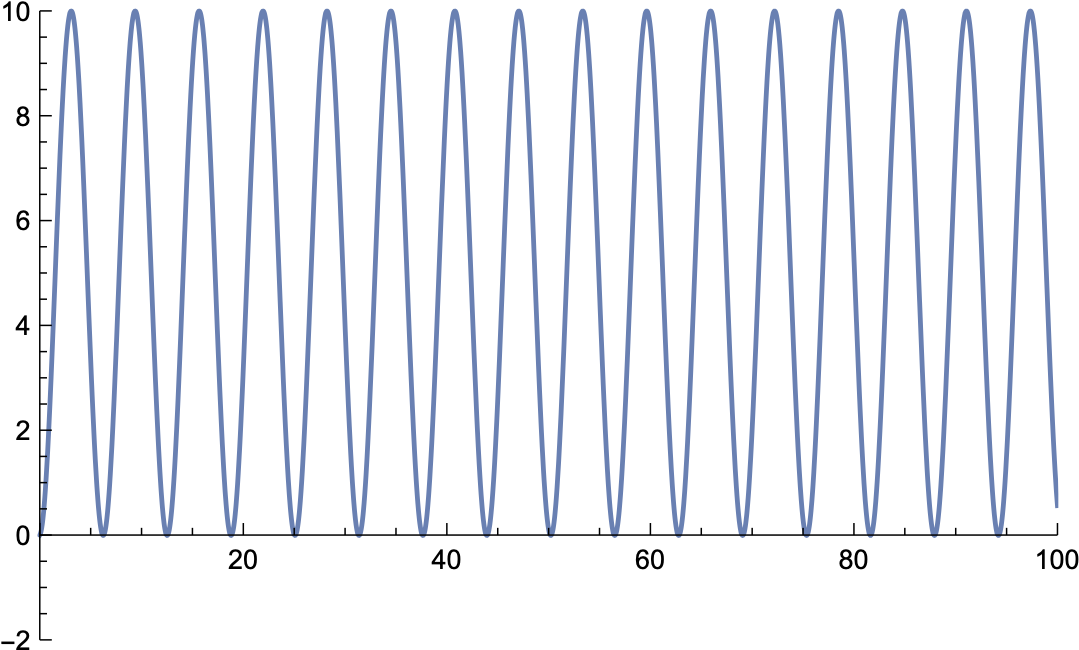
\includegraphics[width=10cm] {x.png}
\caption{$k=0.5,\omega=1,t=0.1$时$<x(t)>$的理论曲线}      
\end{figure}

\begin{figure}[!htbp]   
\centering
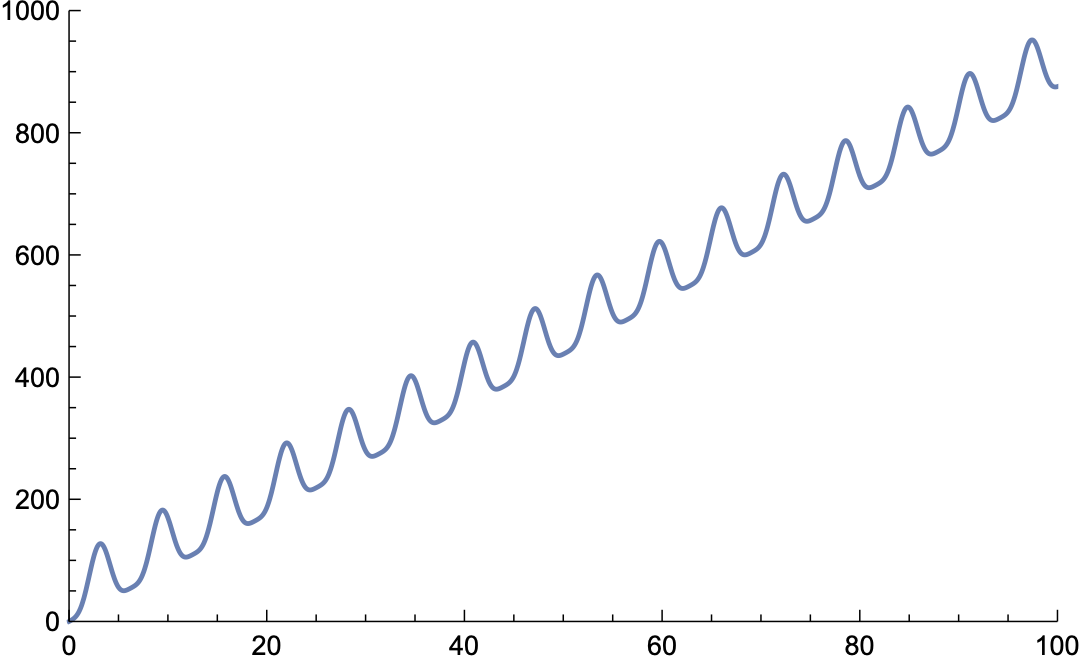
\includegraphics[width=10cm] {x2.png}
\caption{$k=0.5,\omega=1,t=0.1$时$<x^{2}(t)>$的理论曲线}      
\end{figure}


\newpage 当我们选取$k=0$时,此时相当于自由的一维布朗粒子,有程序结果:


	

\begin{figure}[!htbp]   
\centering     
\subfigure[粒子的平均位置]{
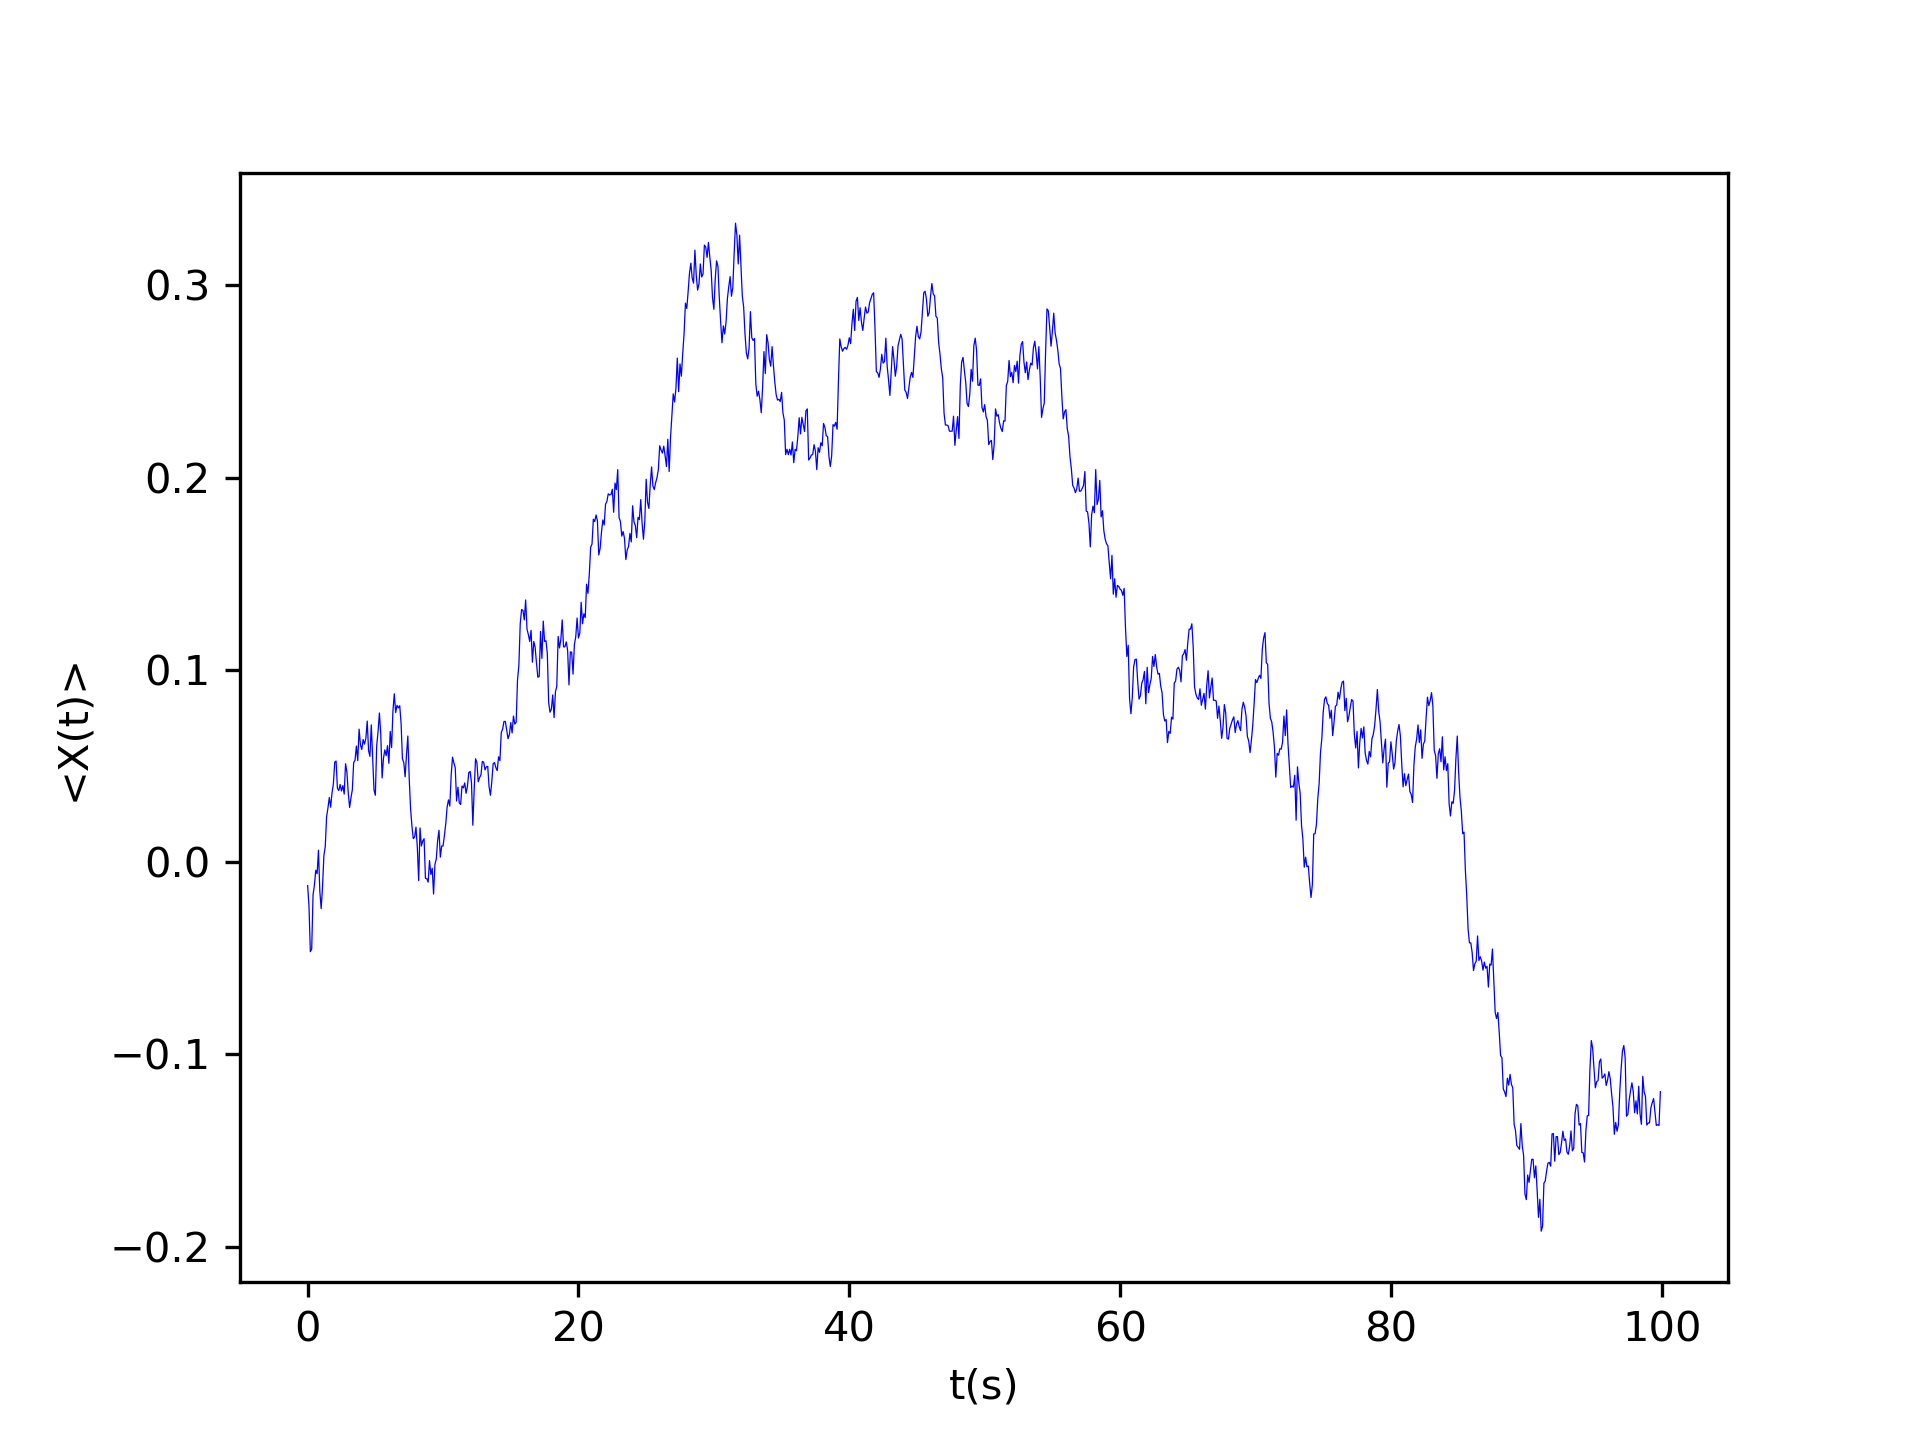
\includegraphics[width=6cm] {w=1/0.png}
}
\subfigure[粒子距离原点距离平方的平均]{
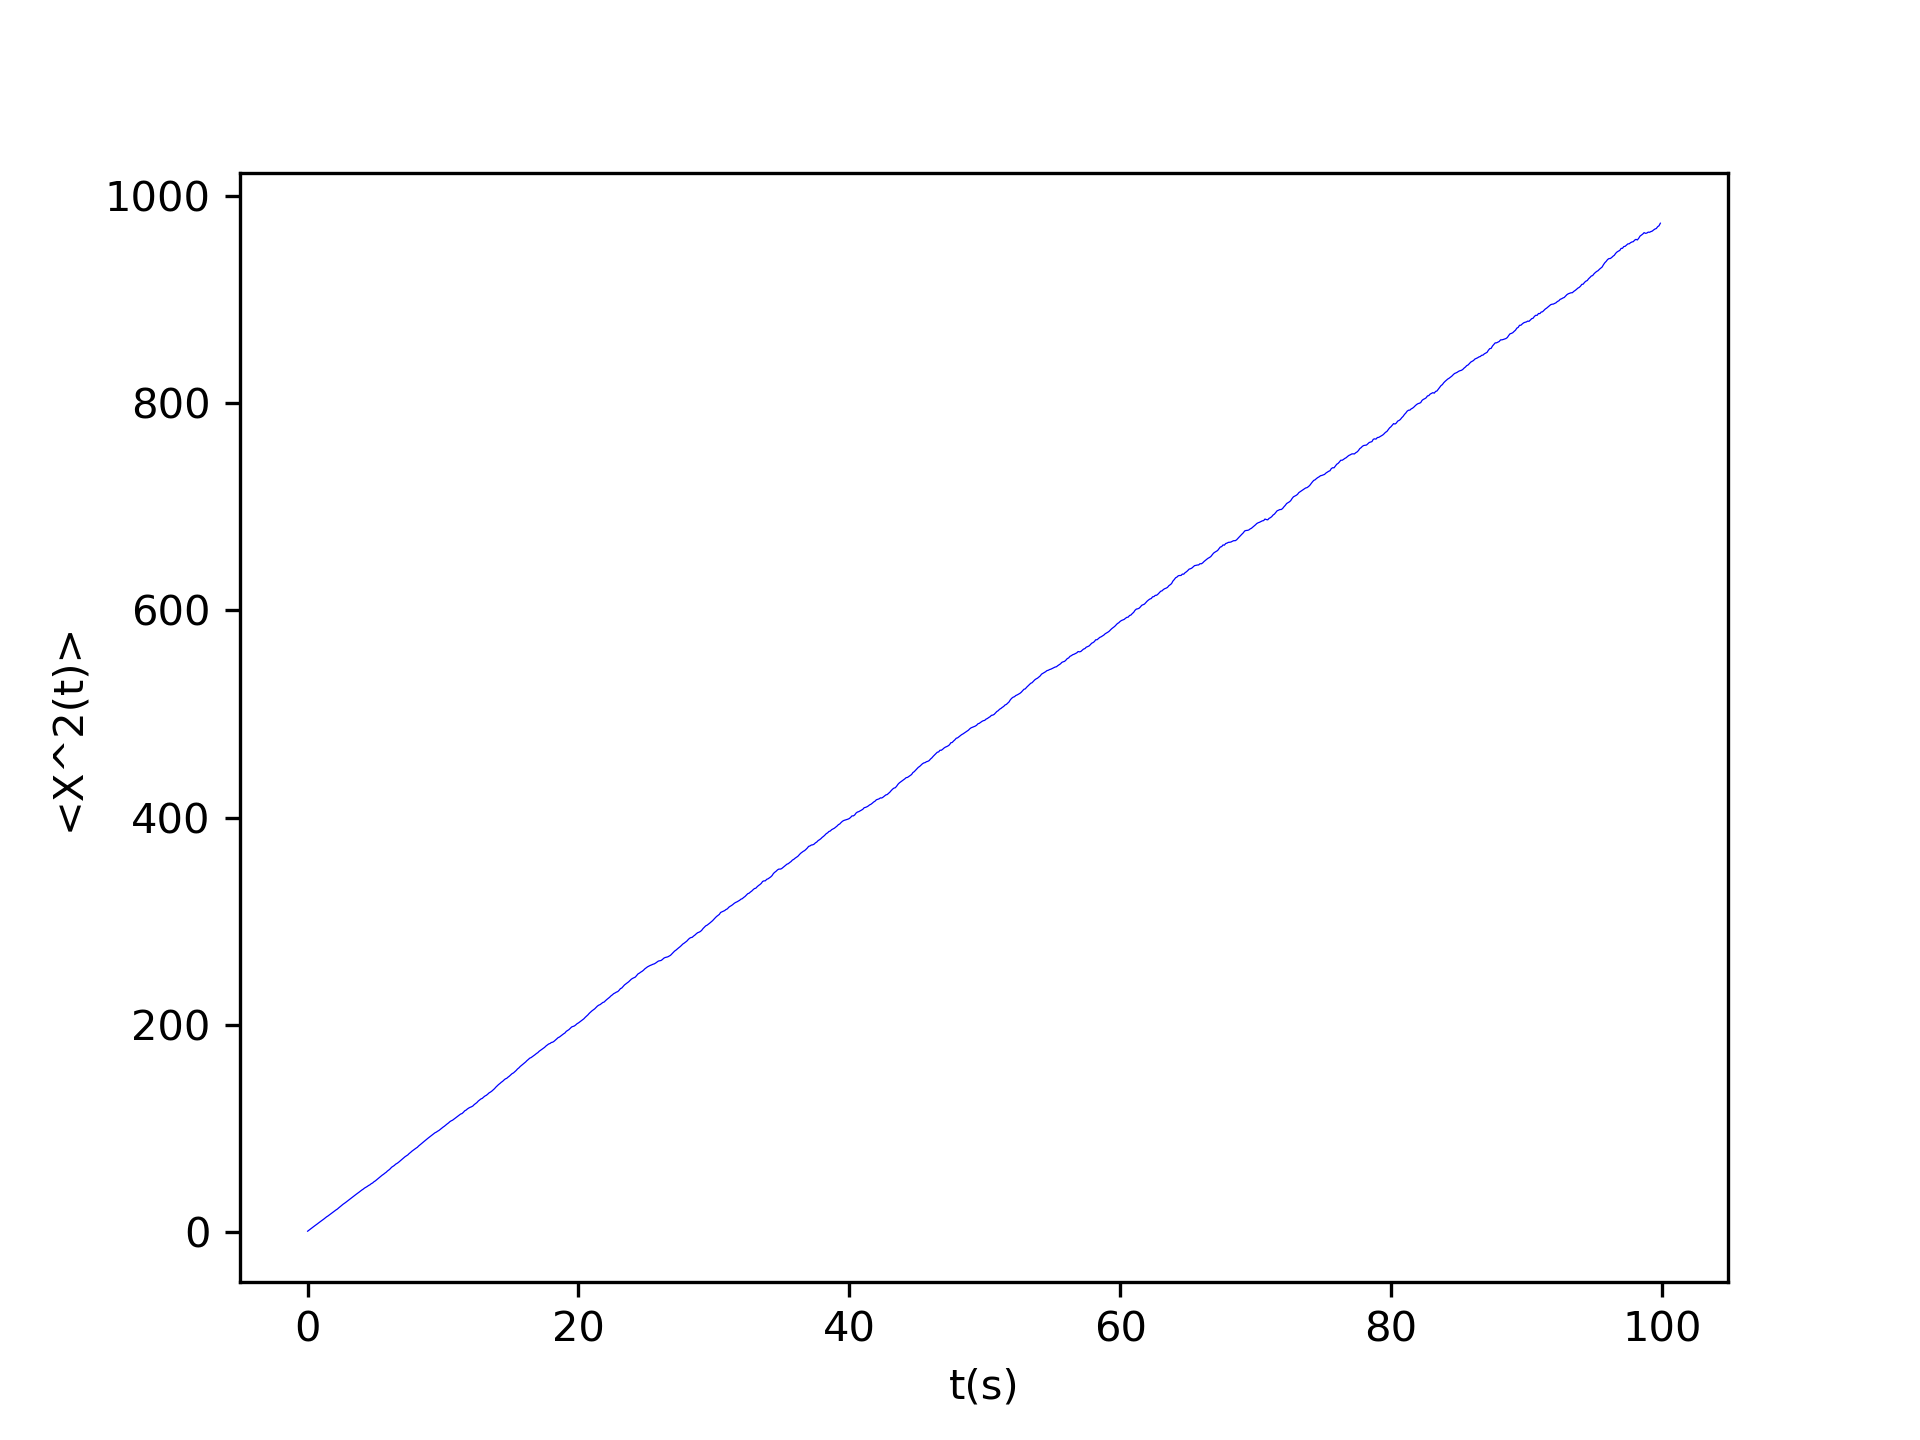
\includegraphics[width=6cm] {w=1/0-2.png}
}            
\caption{$k=0$时模拟10000个粒子行走1000步}      
\end{figure}


可以看出粒子的平均位置在模拟步数内,均比较接近于0,表现出布朗粒子的特性。而从结果上也能看出距离原点距离平方的平均与步数成正比关系,验证了布朗粒子的特性。

对于模拟的5个粒子有:
\begin{figure}[!htbp]
\centering
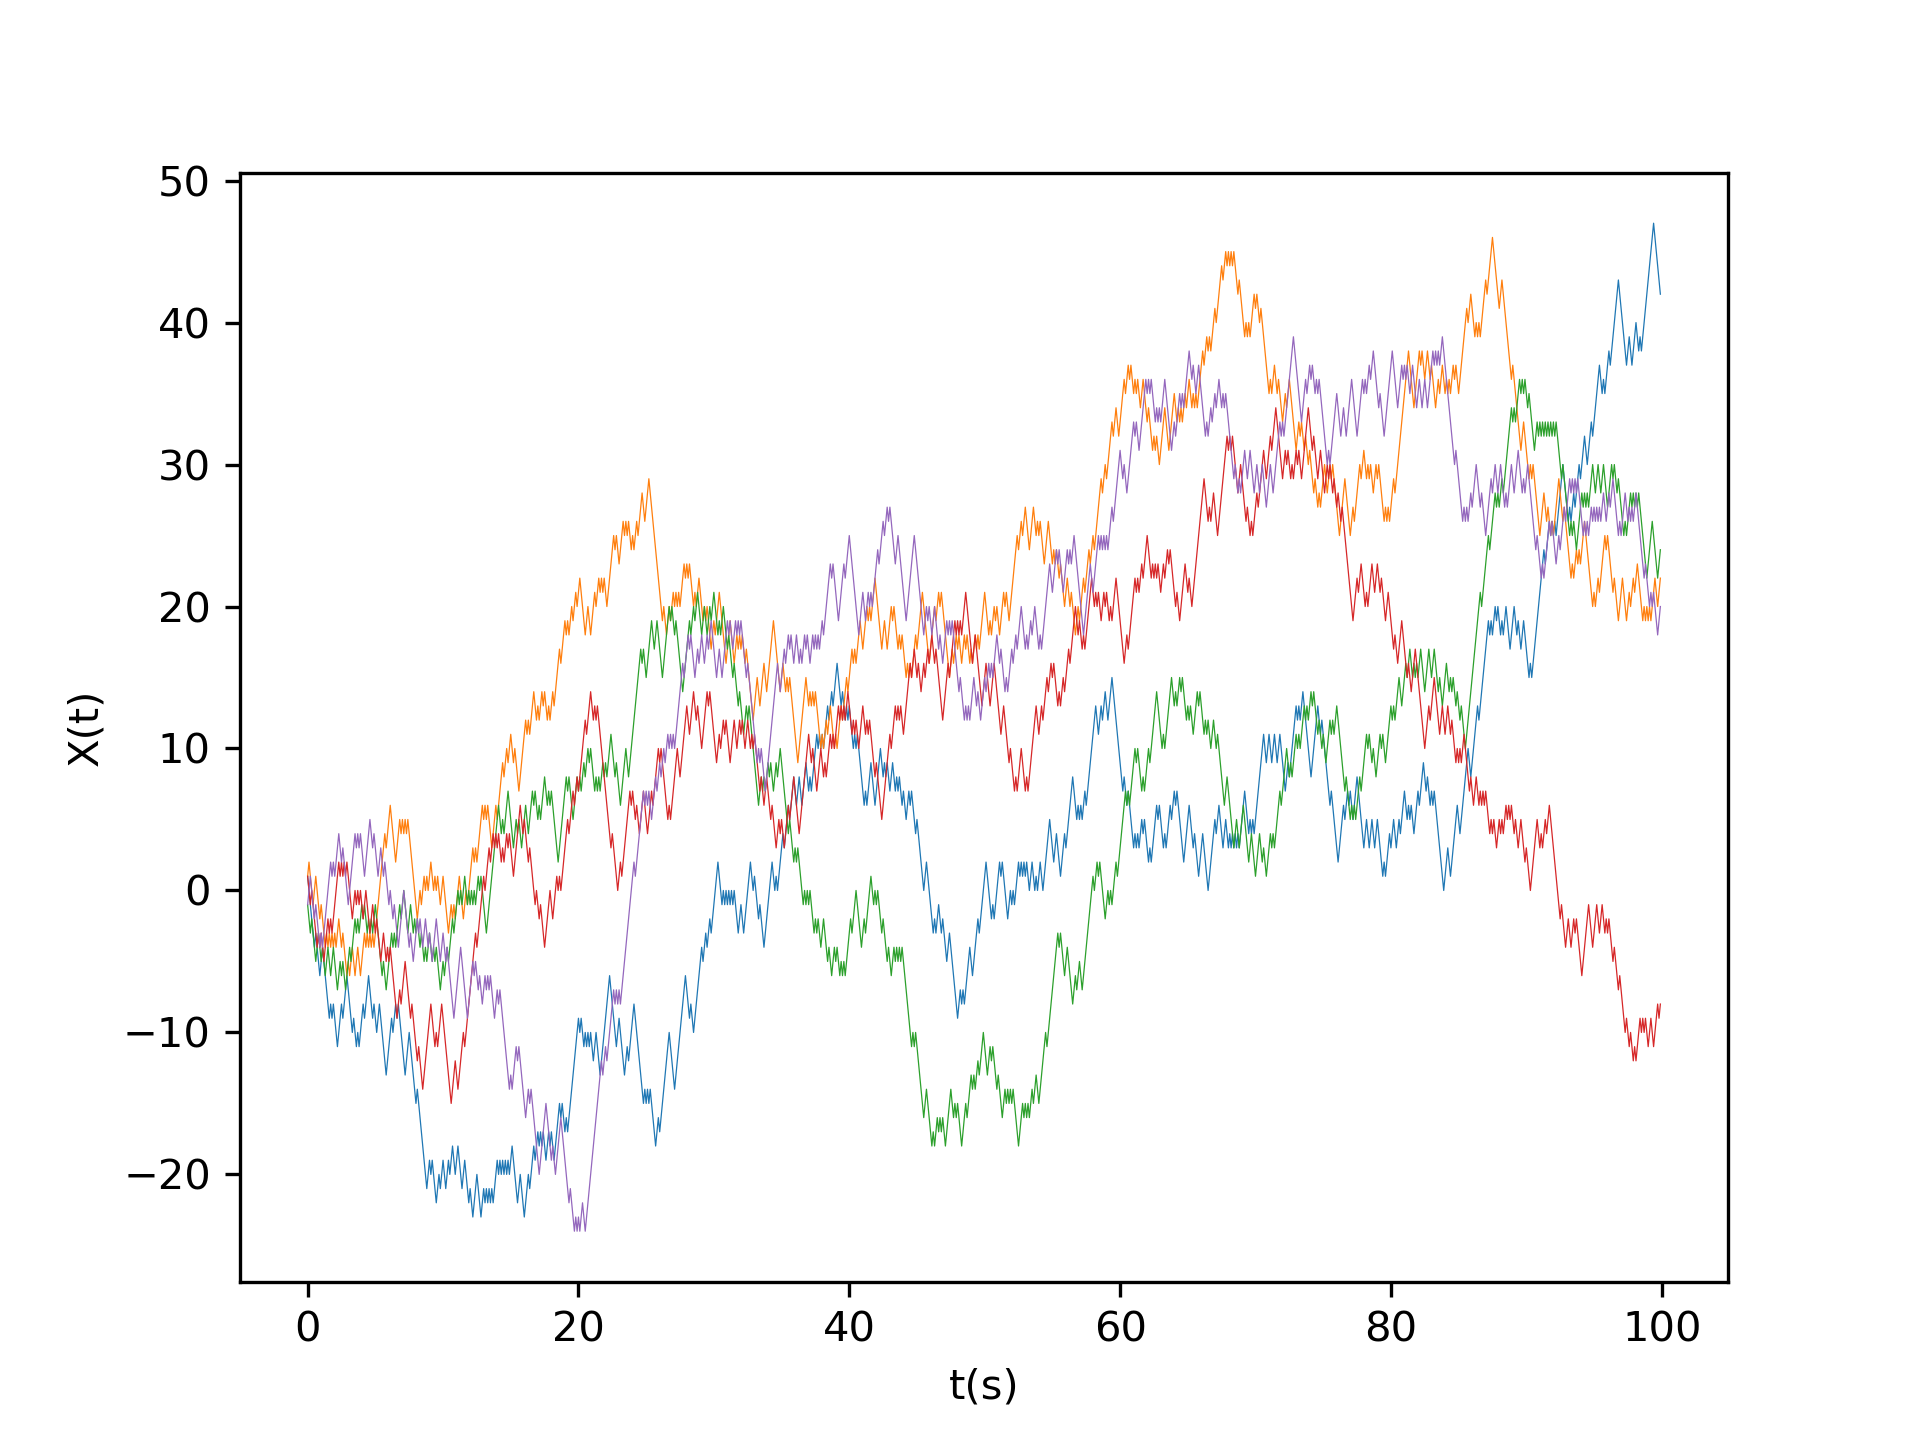
\includegraphics[width=7cm]{w=1/k=0,w=1.png}    	
\caption{$k=0$时5个粒子的运动位置模拟结果}
\end{figure}

当我们设定$k=0.5$时,有:


\begin{figure}[!htbp]   
\centering     
\subfigure[粒子的平均位置]{
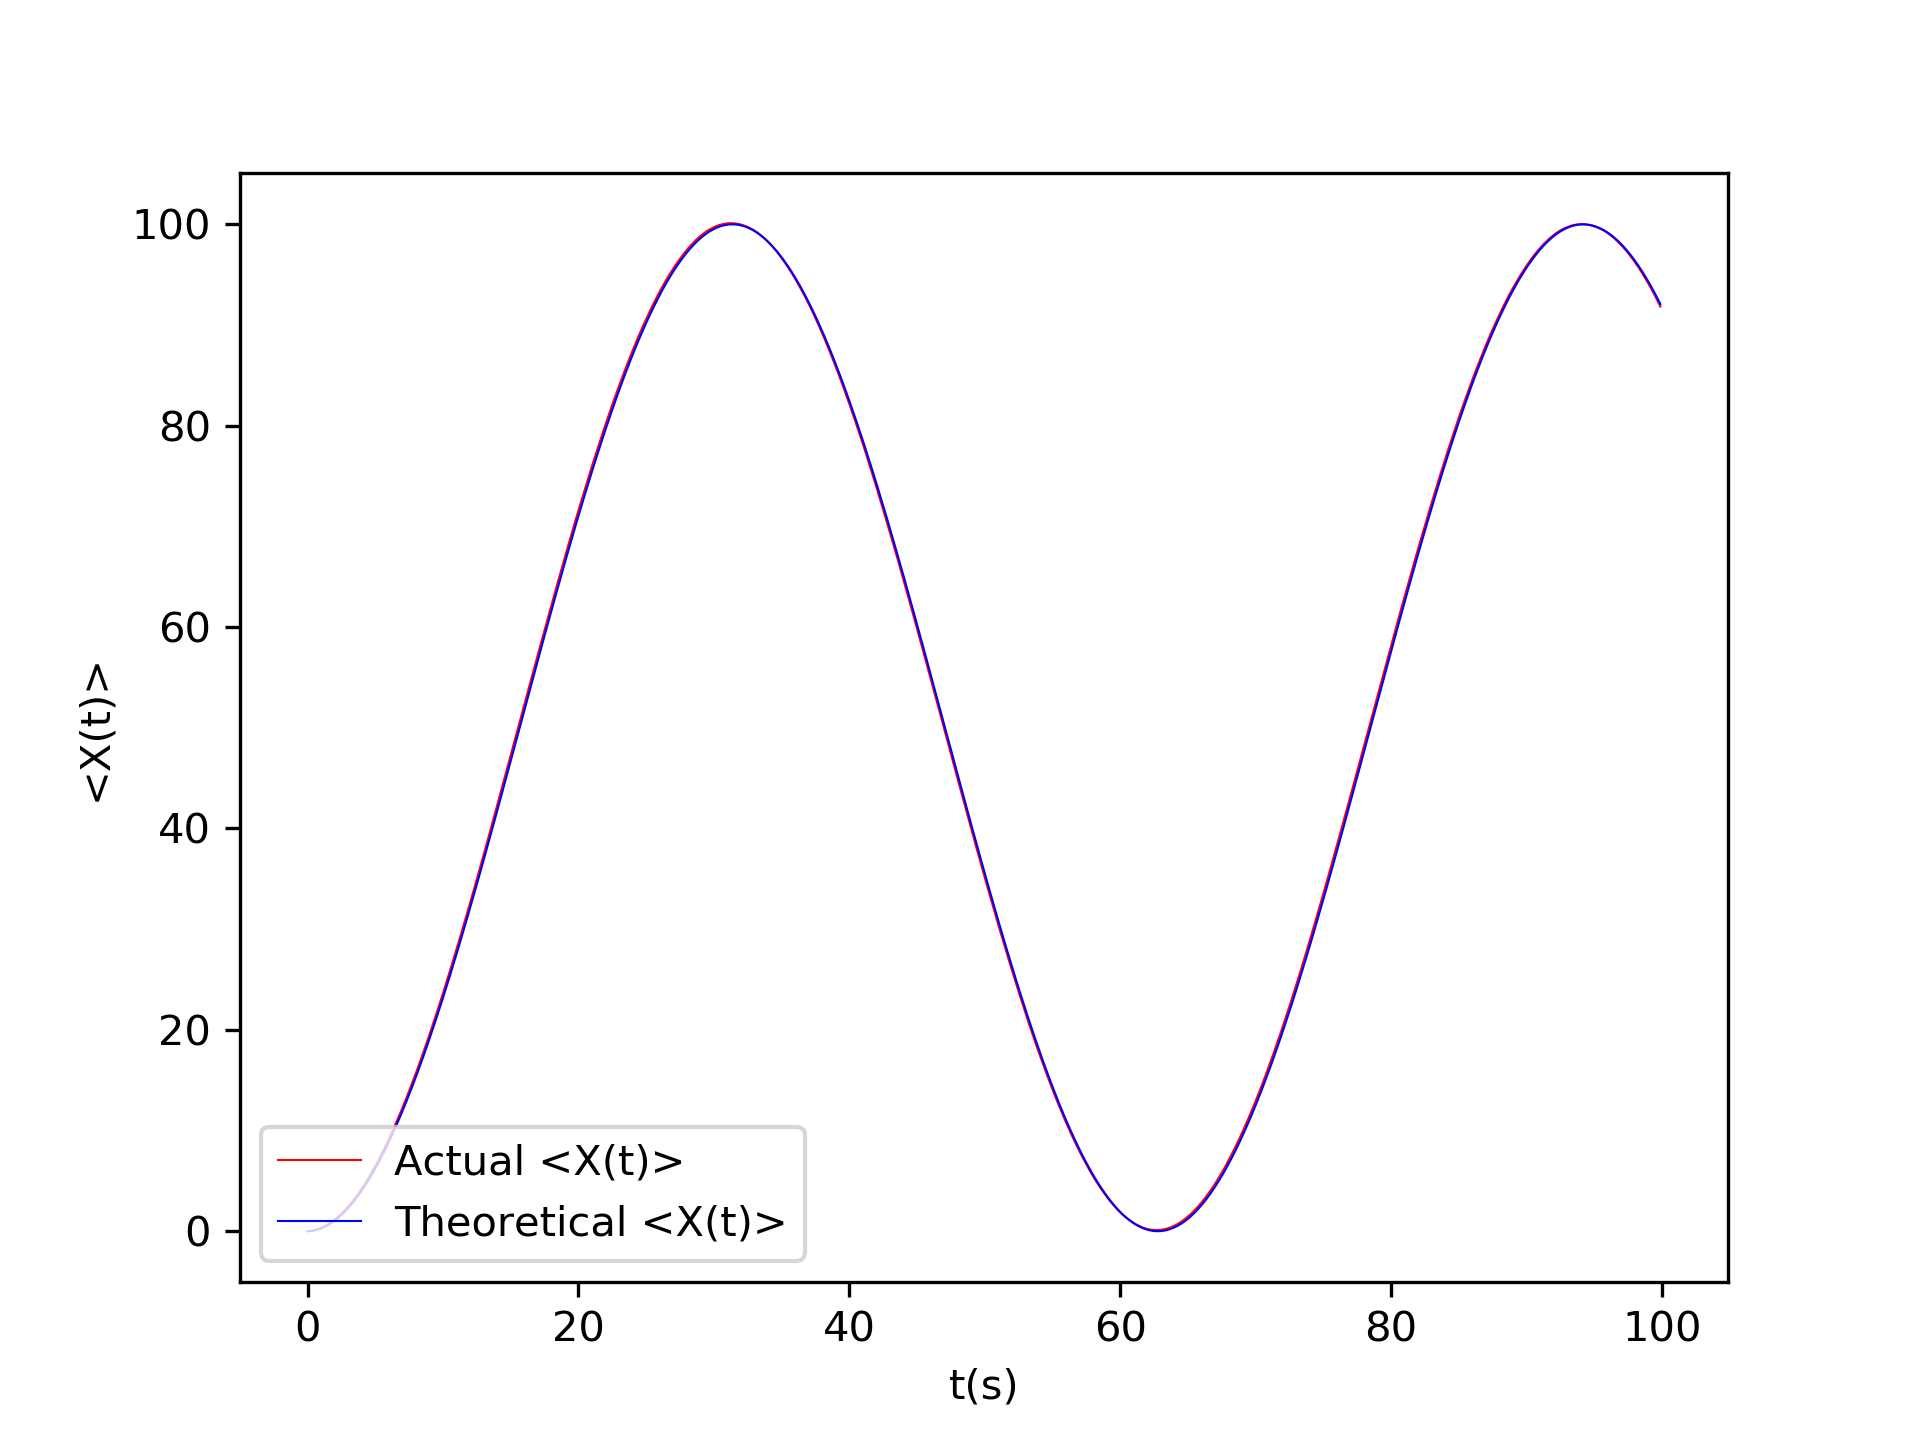
\includegraphics[bb= 0 0 450 370,width=6cm] {w=0.1/k=0.5-1.png}
}
\subfigure[粒子距离原点距离平方的平均]{
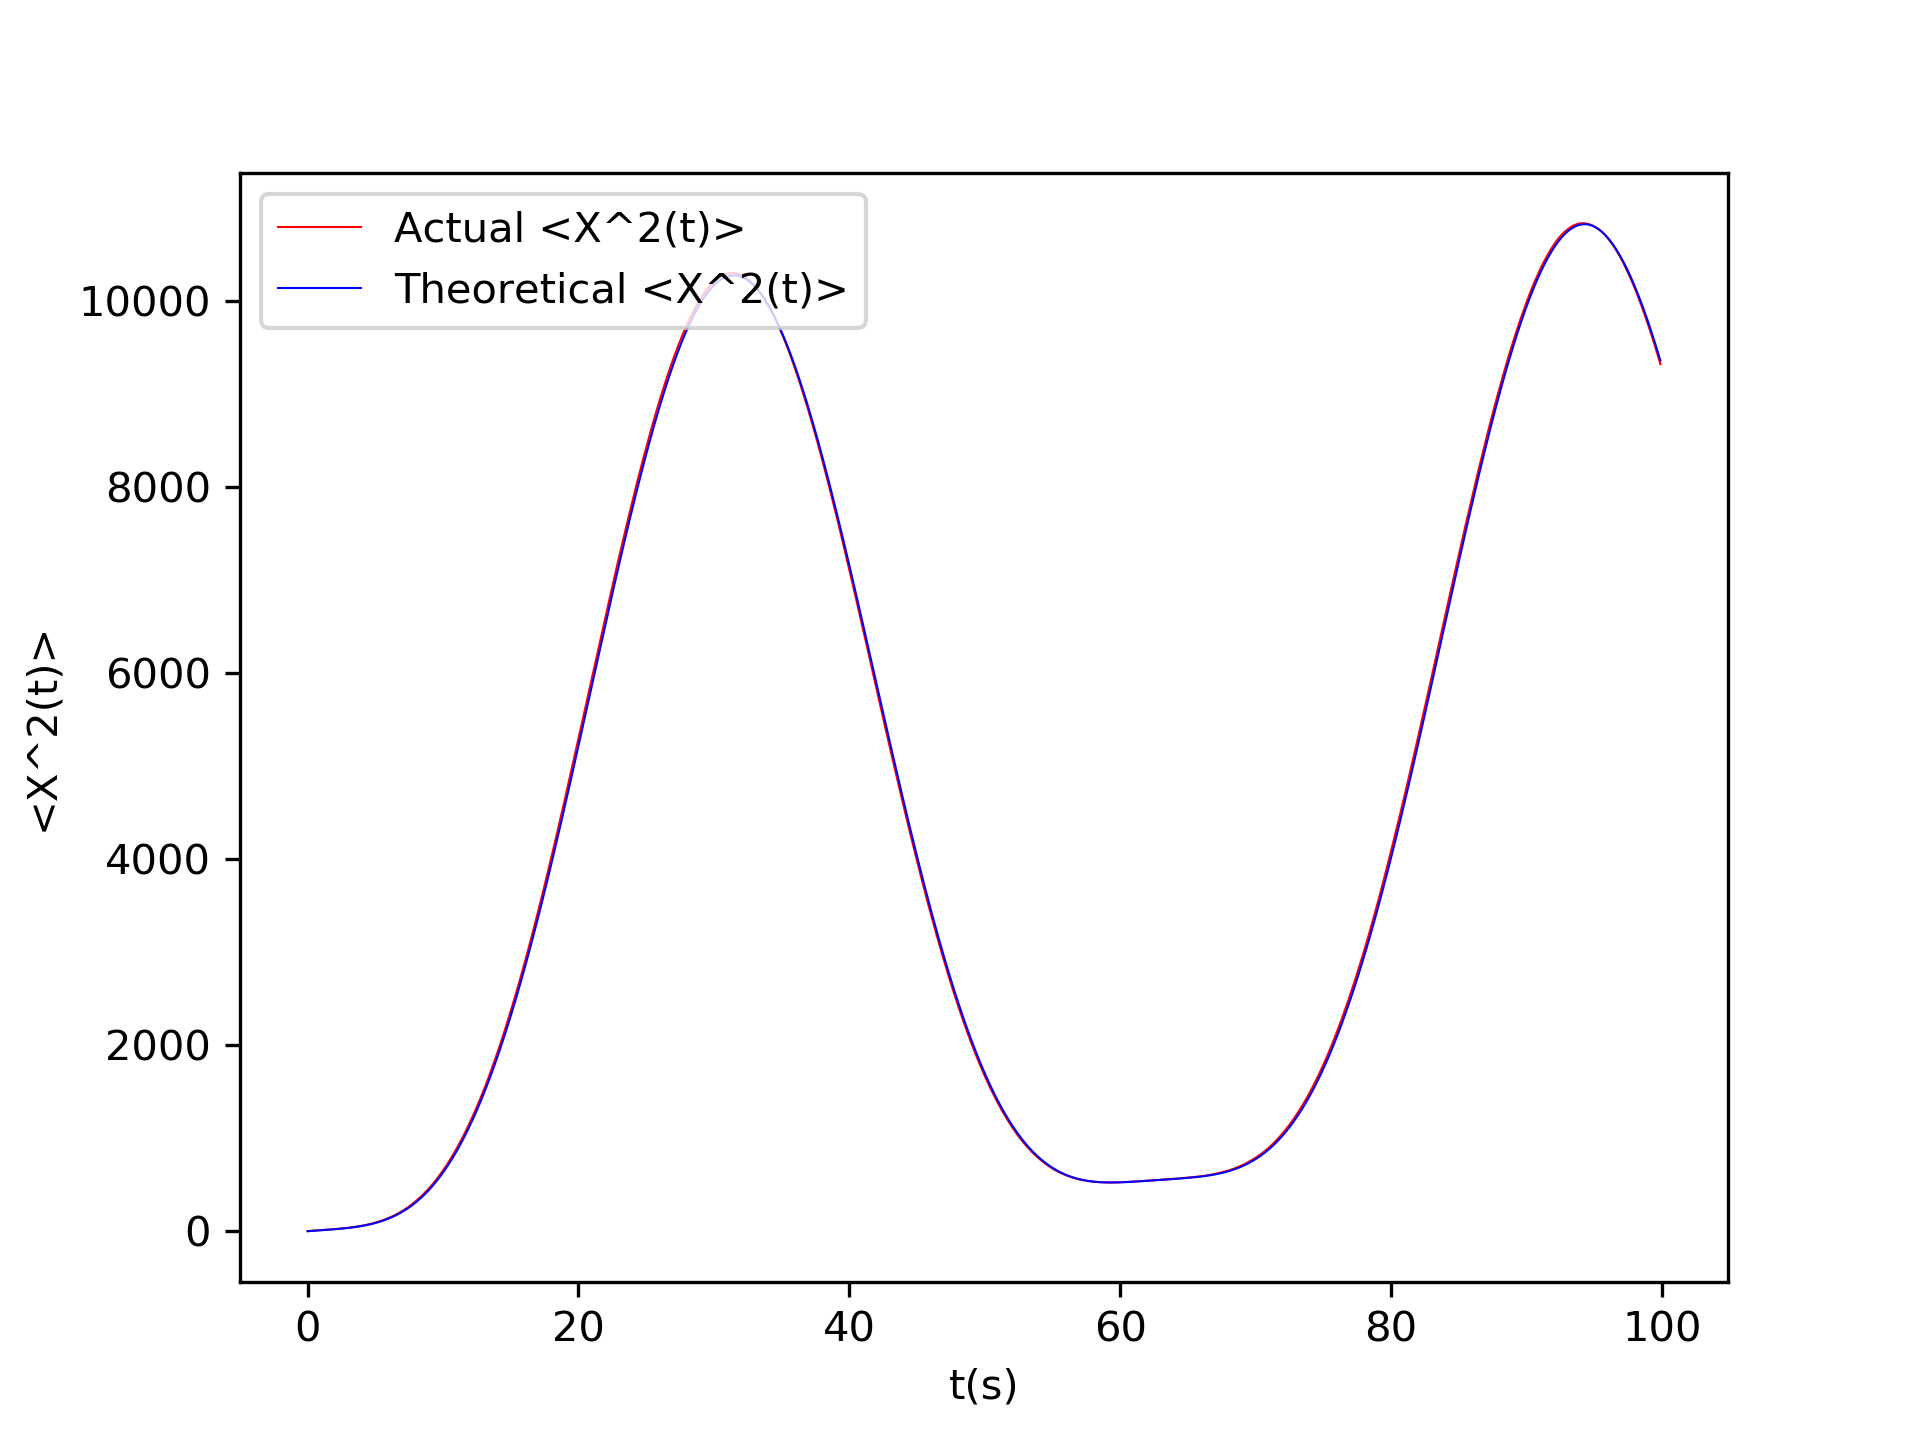
\includegraphics[bb= 0 0 450 370,width=6cm] {w=0.1/k=0.5-2.png}
}            
\caption{$k=0.5,\omega=0.1$时模拟100000个粒子行走1000步}      
\end{figure}


\begin{figure}[!htbp]   
\centering     
\subfigure[粒子的平均位置]{
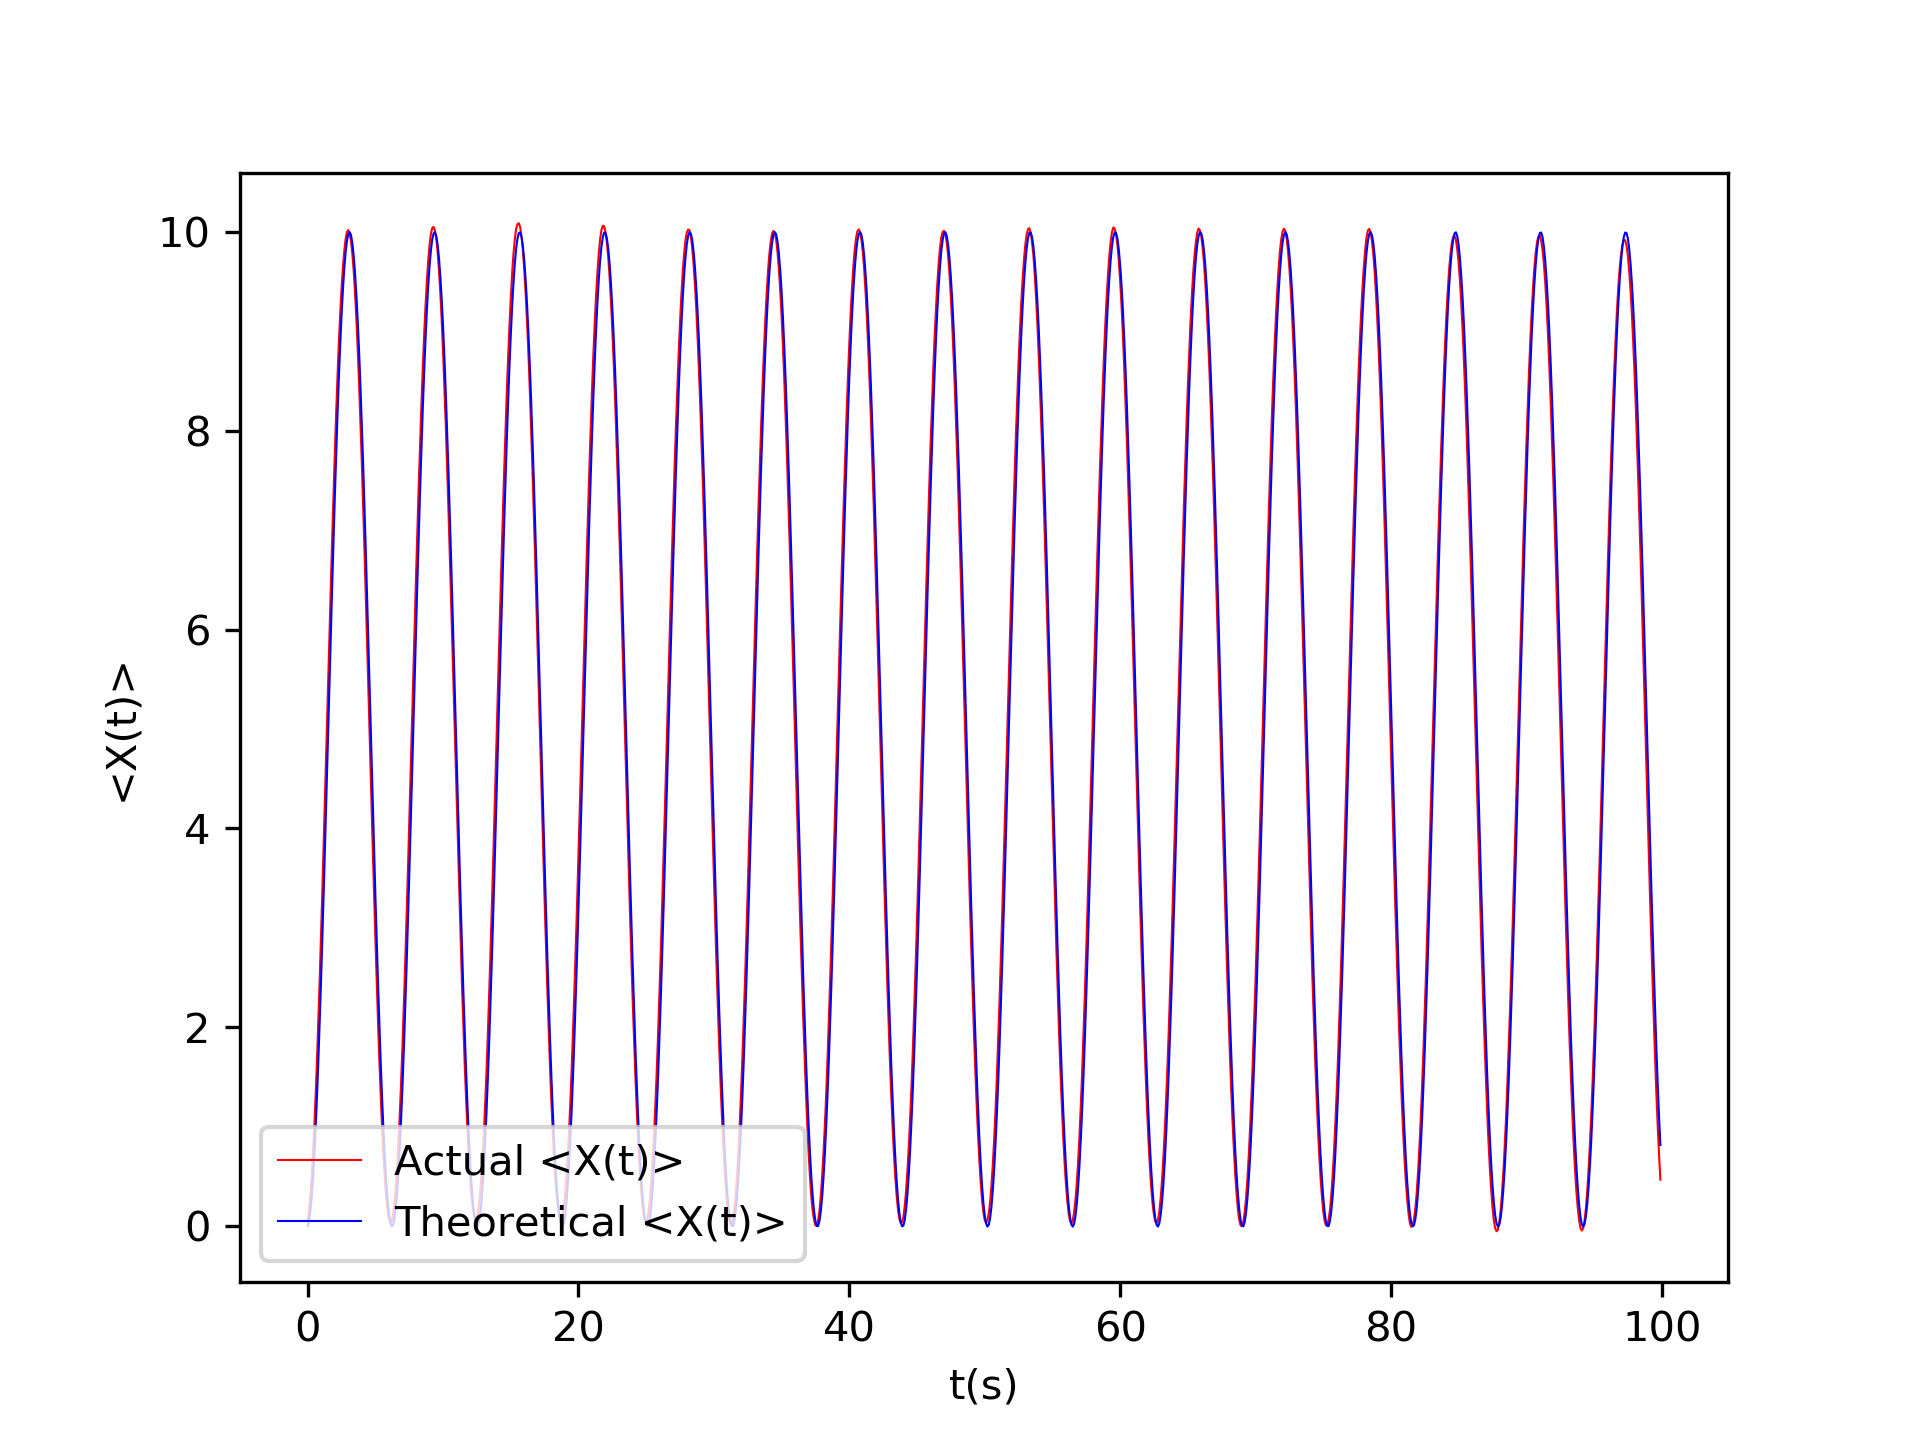
\includegraphics[bb= 0 0 450 370,width=6cm] {w=1/k=0.5-1.png}
}
\subfigure[粒子距离原点距离平方的平均]{
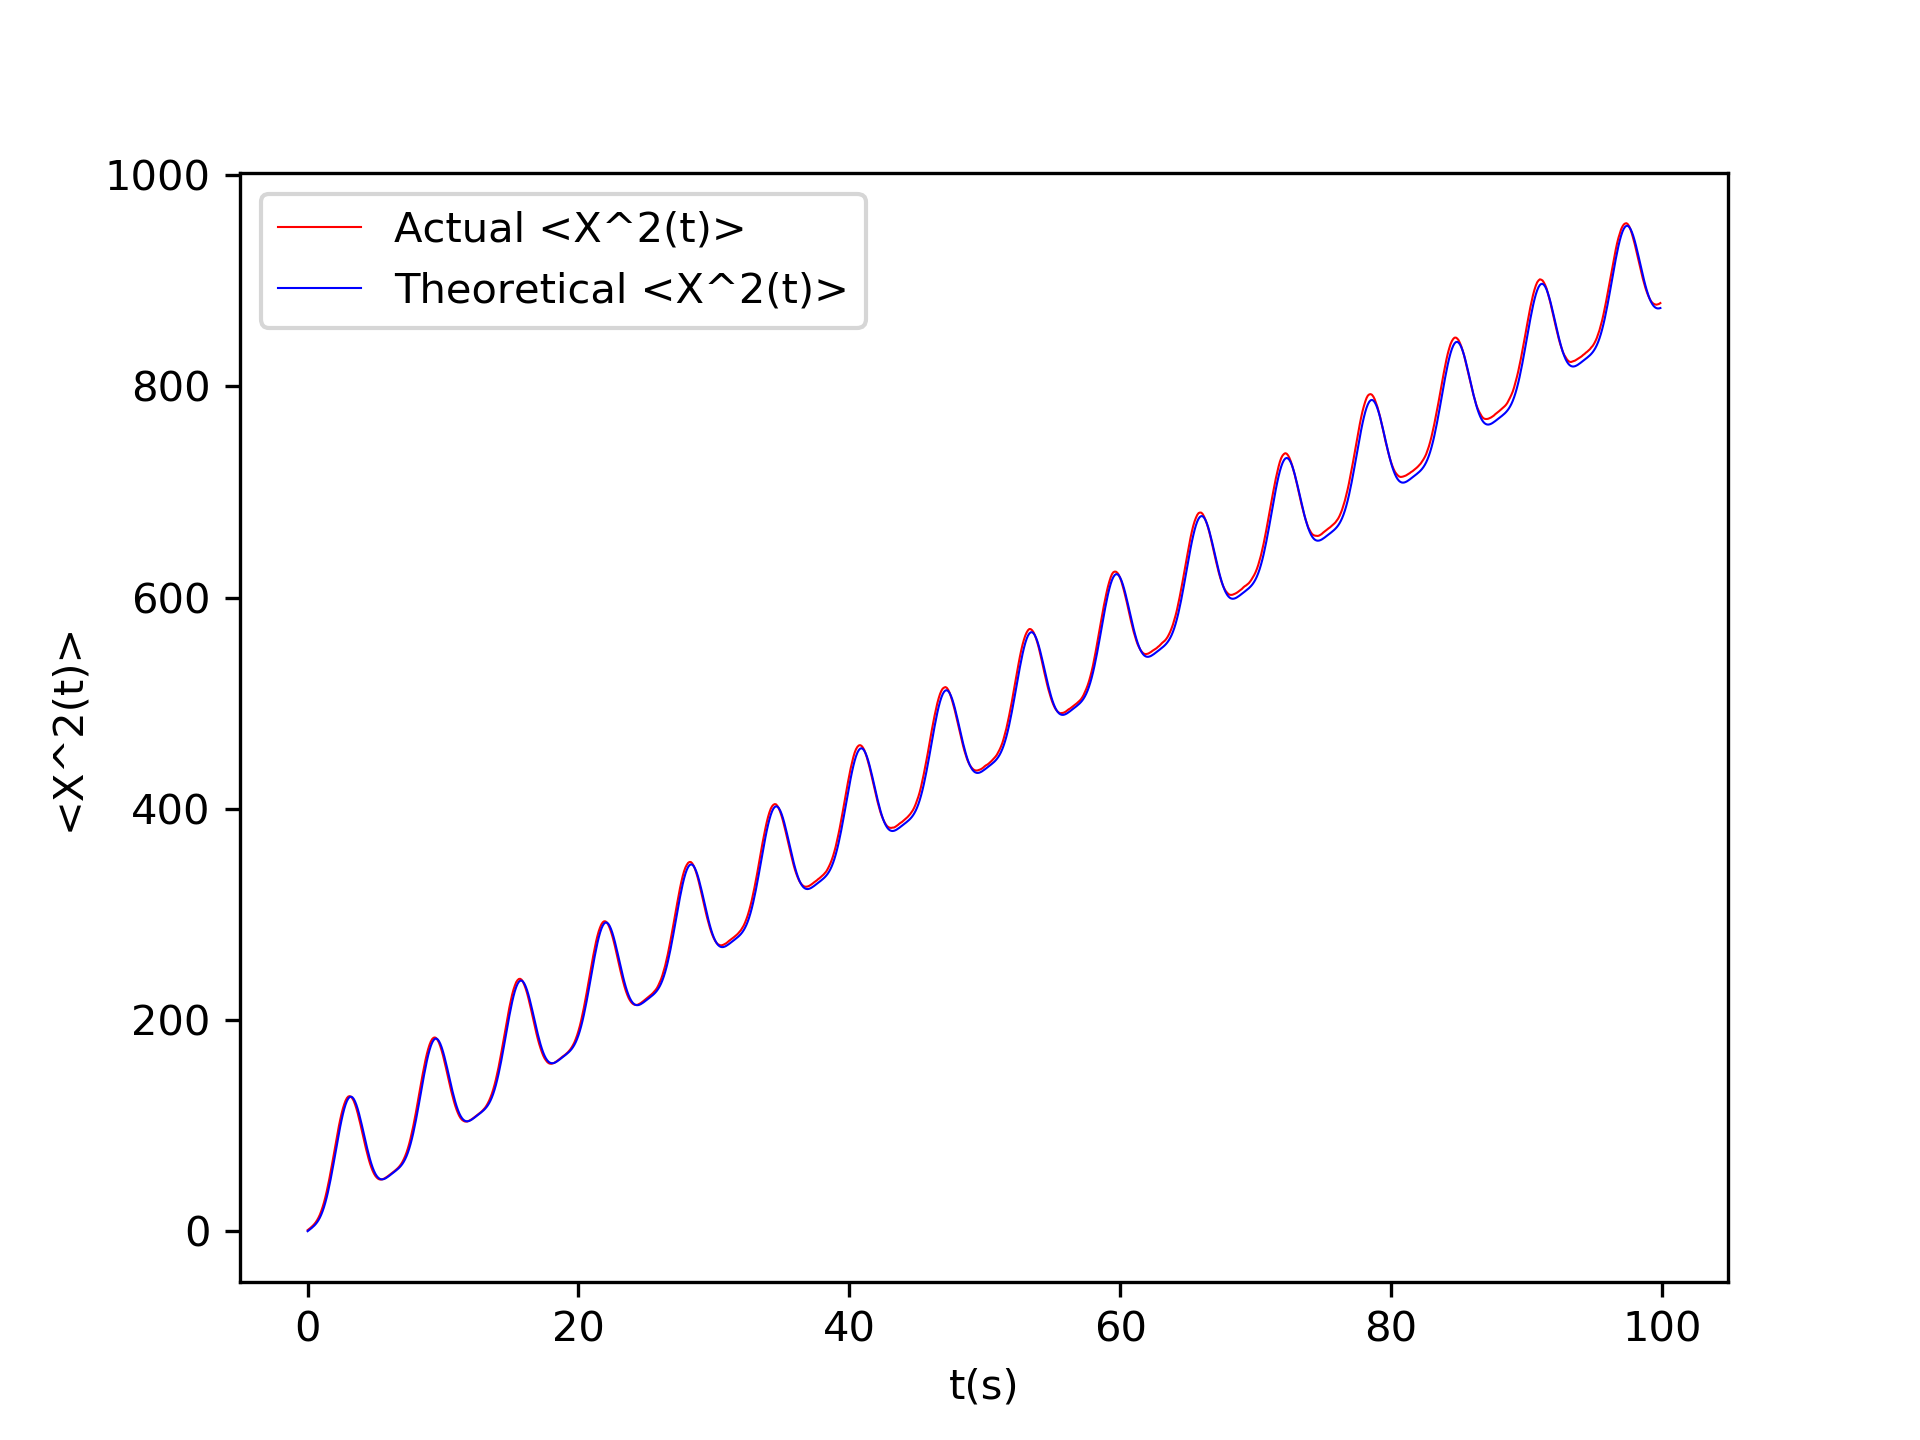
\includegraphics[bb= 0 0 450 370,width=6cm] {w=1/k=0.5-2.png}
}            
\caption{$k=0.5,\omega=1$时模拟100000个粒子行走1000步}      
\end{figure}


\begin{figure}[!htbp]   
\centering     
\subfigure[粒子的平均位置]{
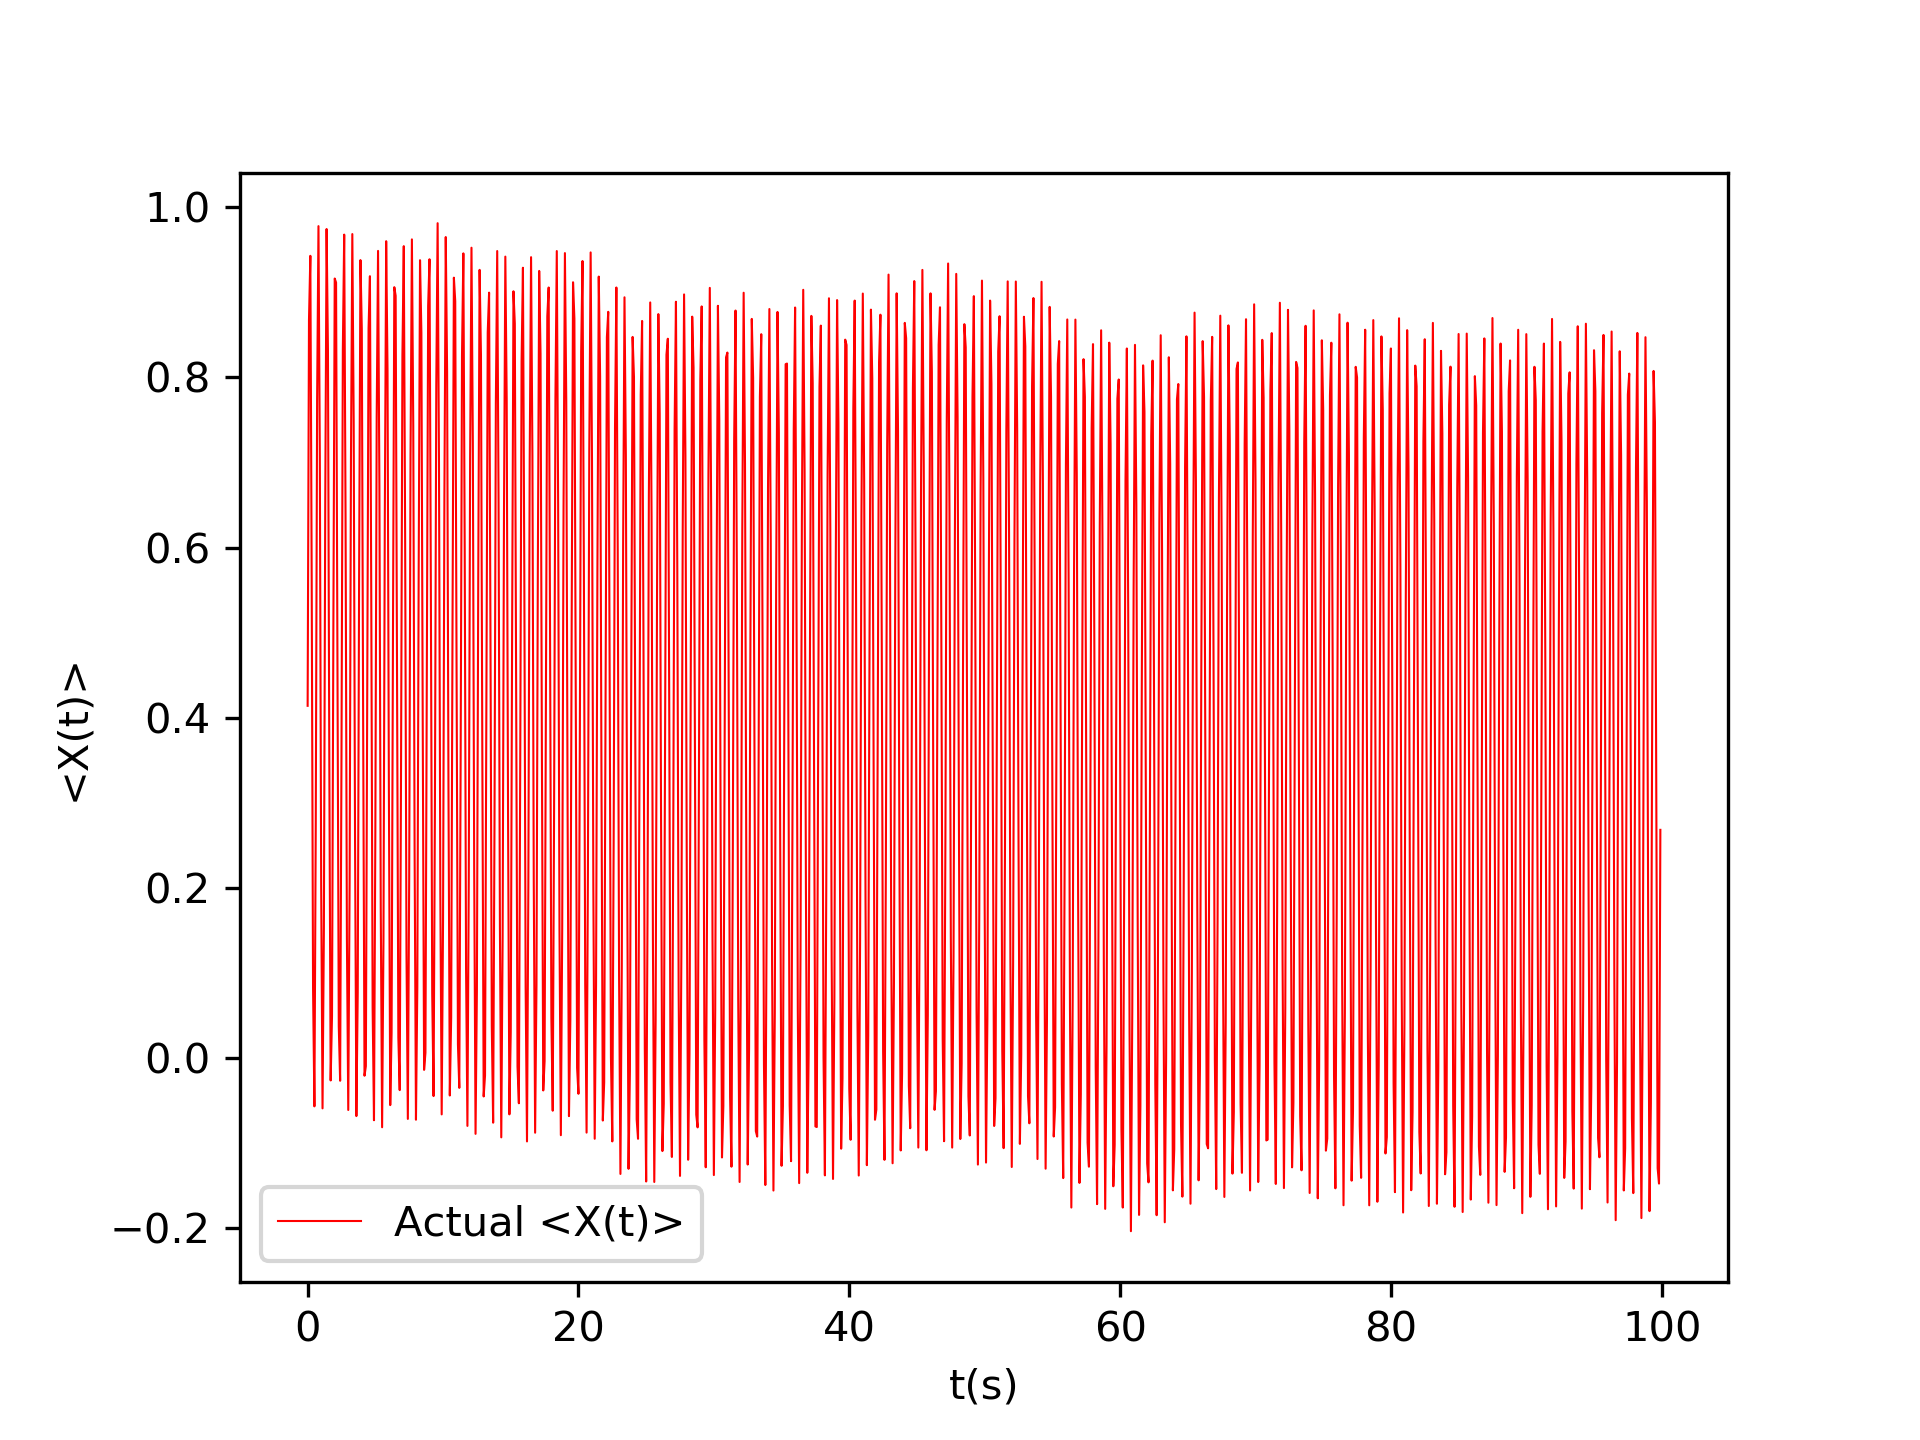
\includegraphics[bb= 0 0 450 370,width=6cm] {w=10/k=0.5-1.png}
}
\subfigure[粒子距离原点距离平方的平均]{
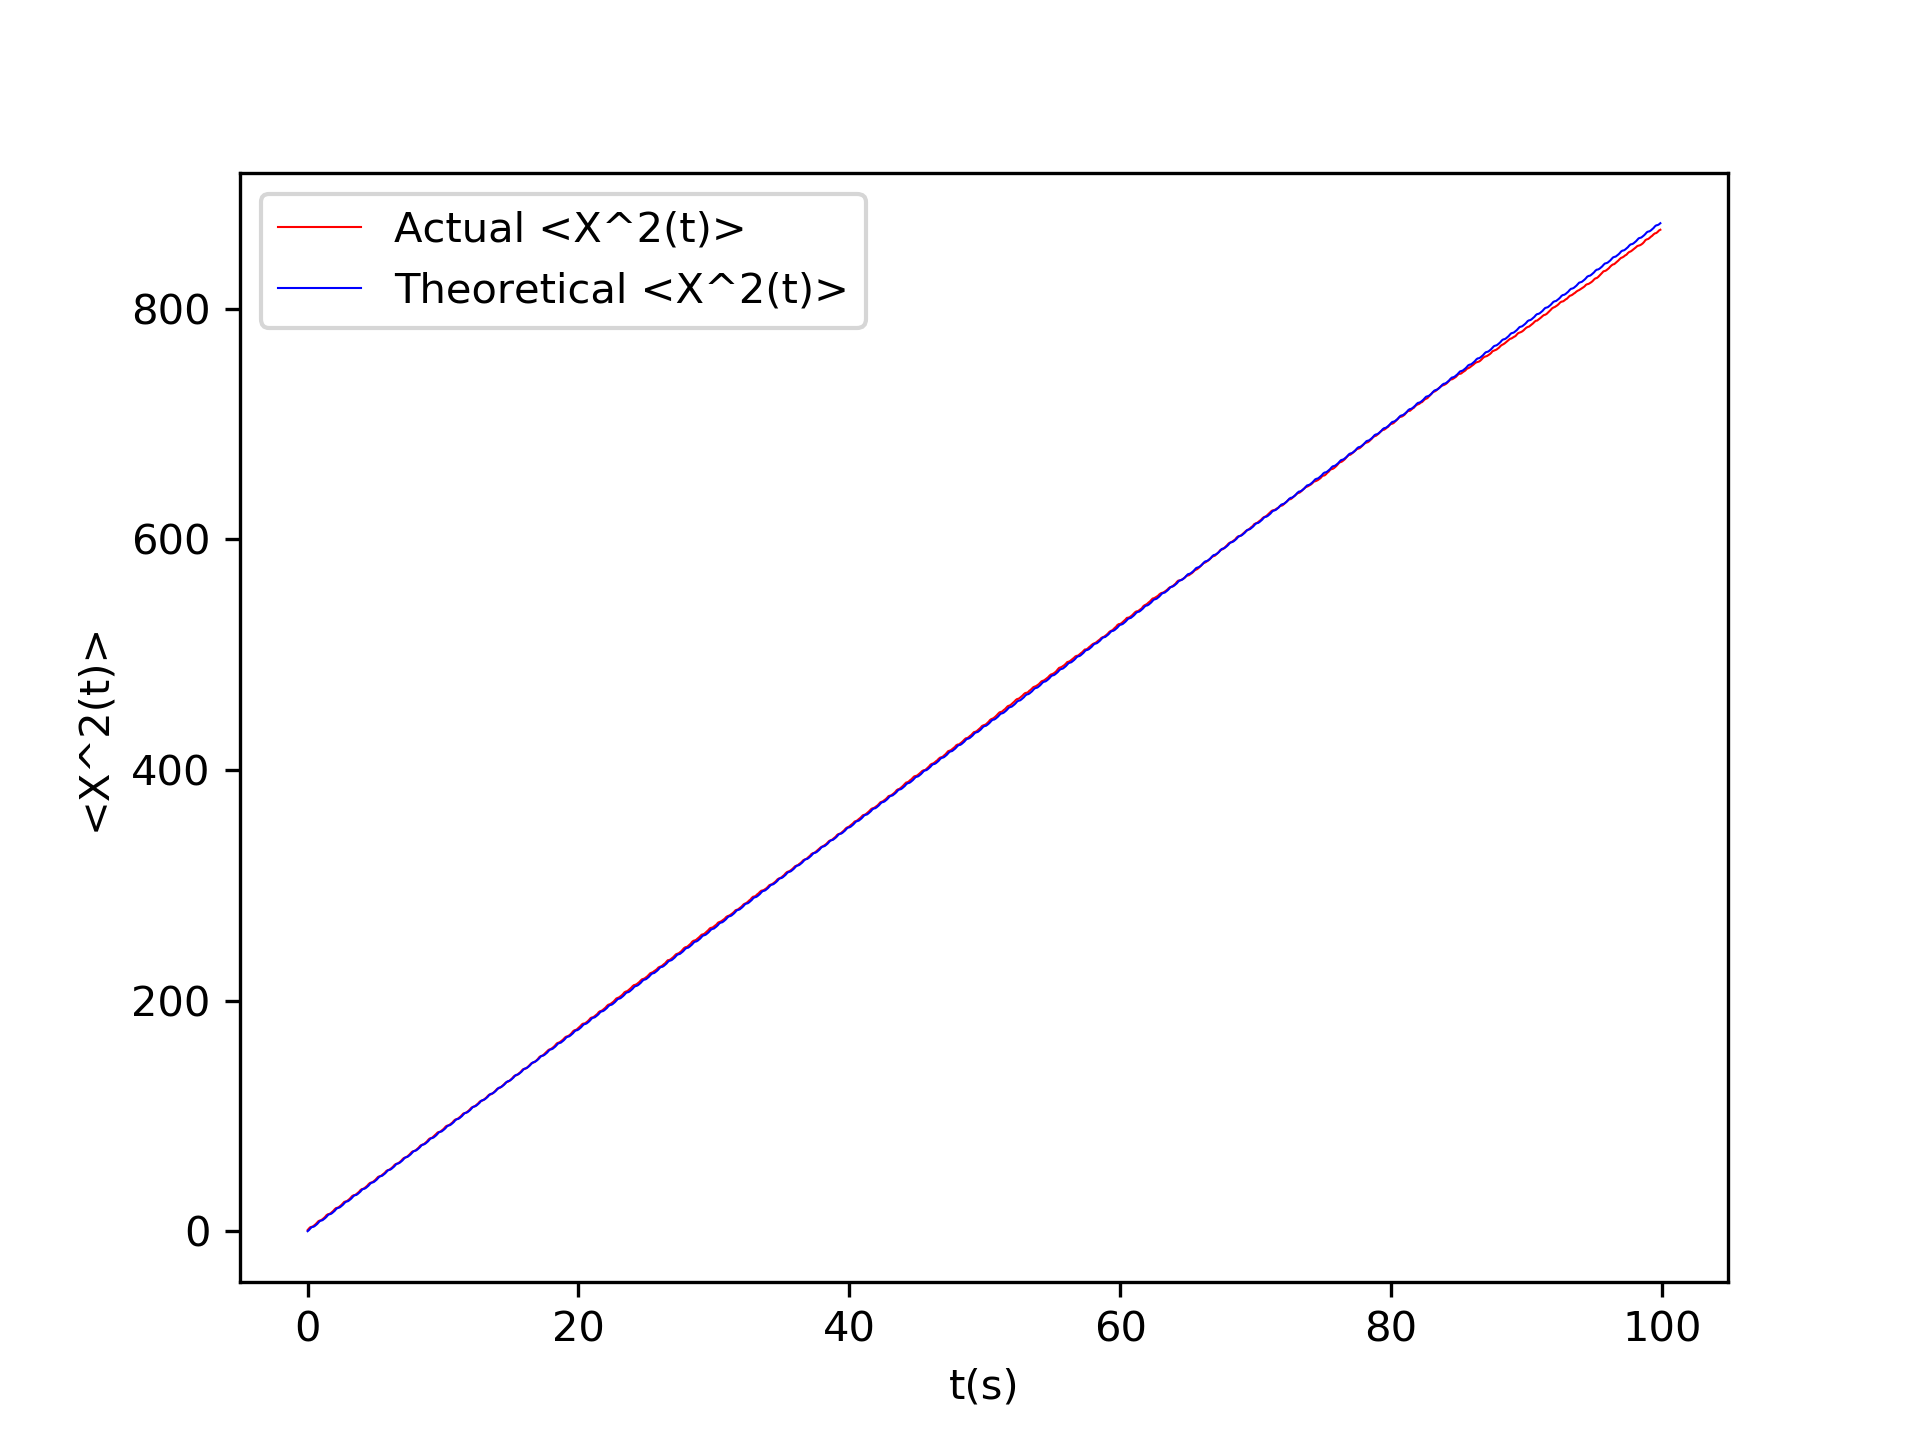
\includegraphics[bb= 0 0 450 370,width=6cm] {w=10/k=0.5-2.png}
}            
\caption{$k=0.5,\omega=10$时模拟100000个粒子行走1000步}      
\end{figure}


\begin{figure}[!htbp]   
\centering     
\subfigure[粒子的平均位置]{
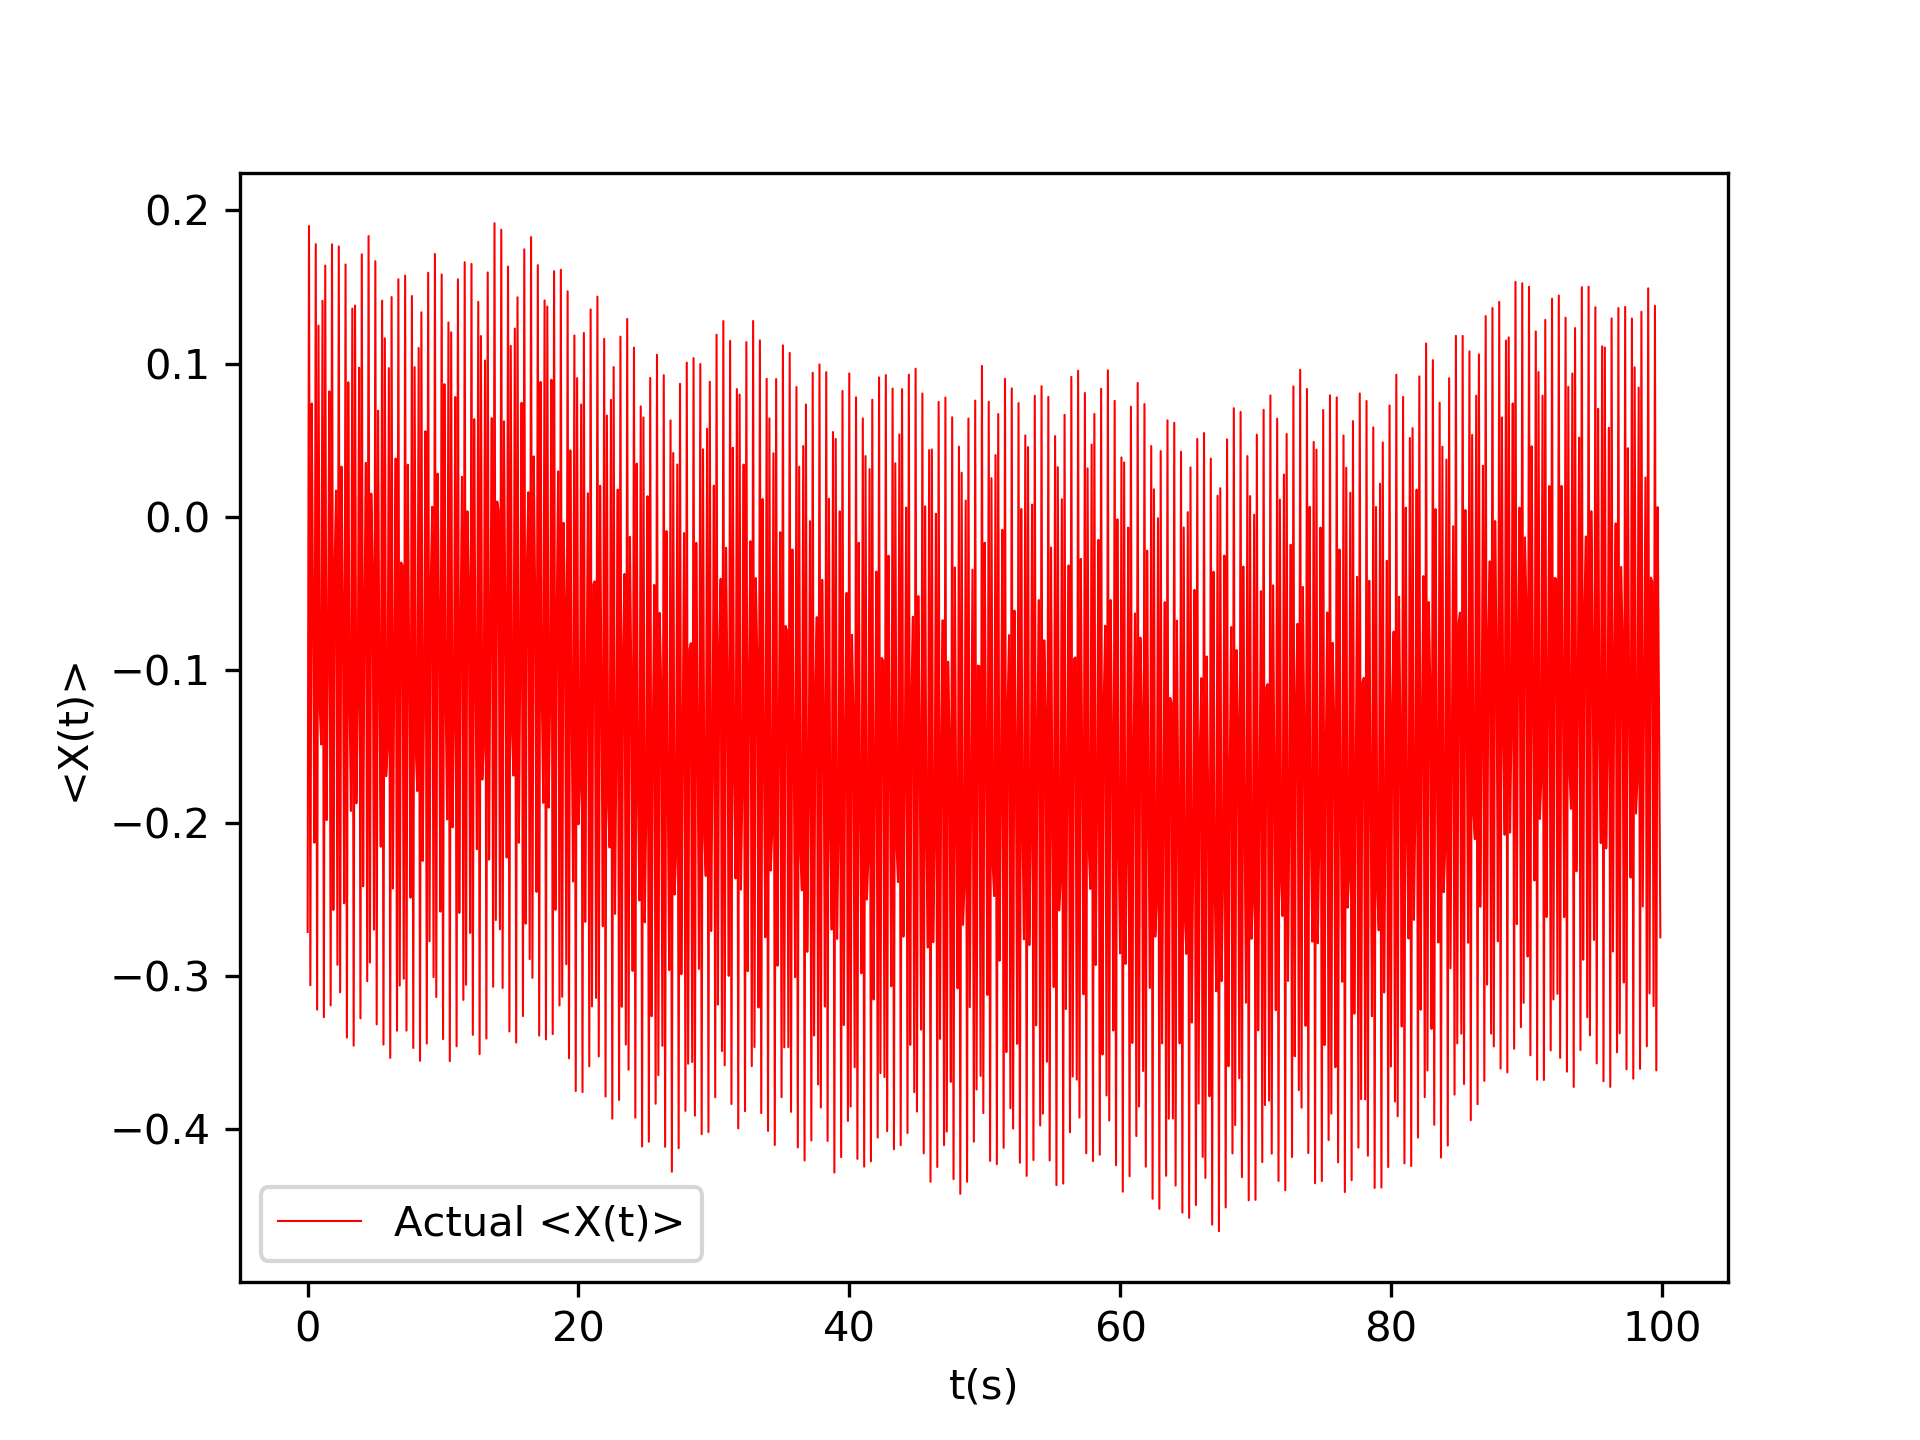
\includegraphics[bb= 0 0 450 370,width=6cm] {w=100/k=0.5-1.png}
}
\subfigure[粒子距离原点距离平方的平均]{
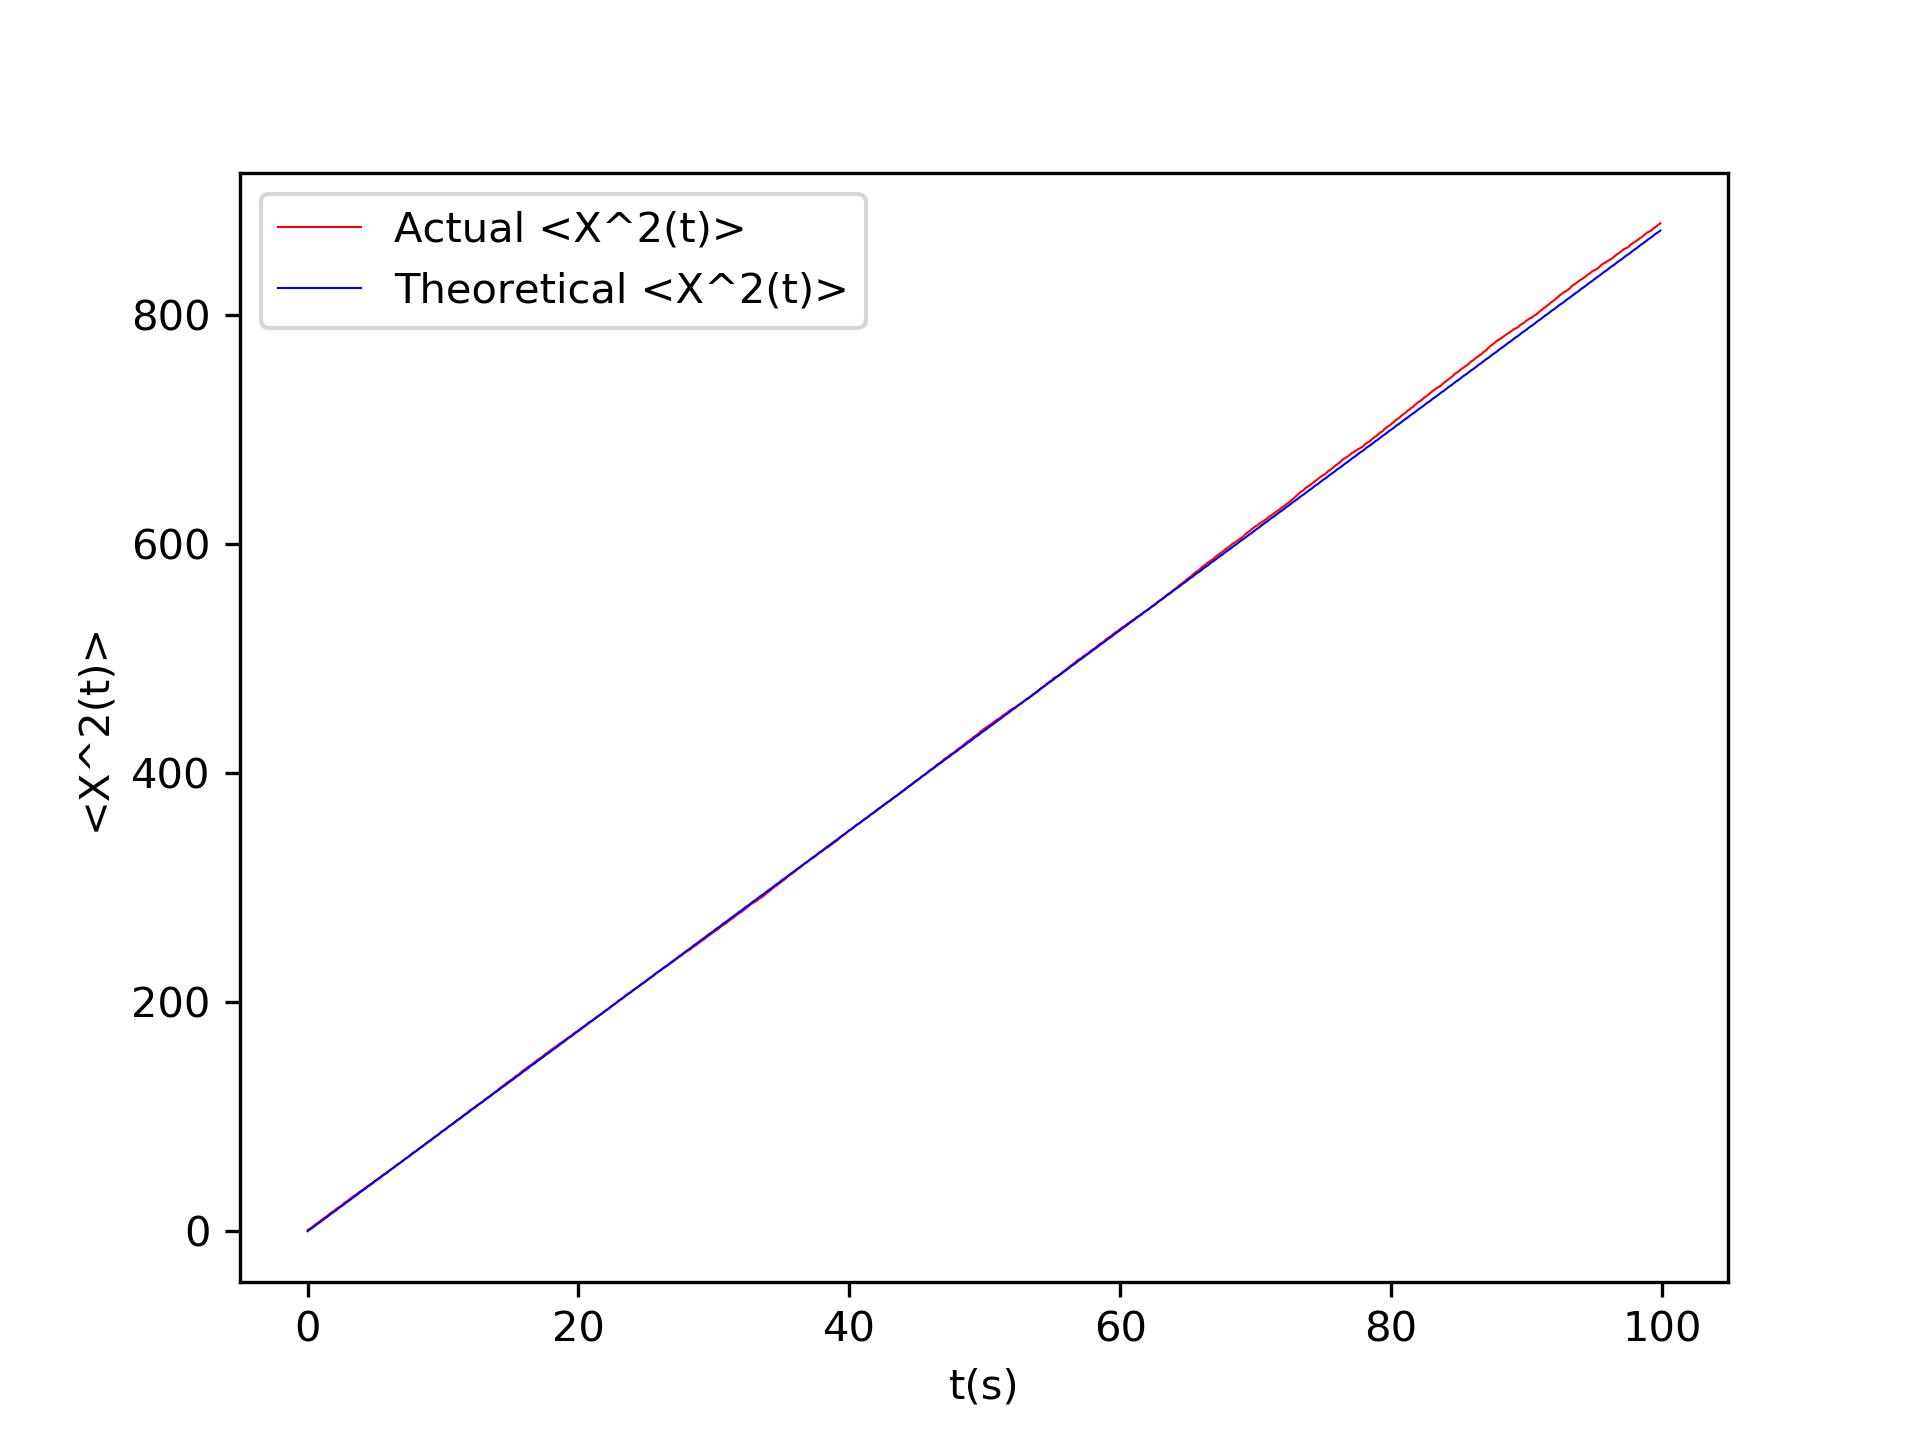
\includegraphics[bb= 0 0 450 370,width=6cm] {w=100/k=0.5-2.png}
}            
\caption{$k=0.5,\omega=100$时模拟100000个粒子行走1000步}      
\end{figure}


\newpage 可以看出在影响因子$k=0.5$时粒子的平均位置已经呈现与正弦力同频率的震荡。而距离原点距离的平方的平均基本为在$k=0$时的线性关系上叠加与正弦力同频率的震荡。两者的震荡幅度均随着正弦力频率的增加而减少,这点也很好理解,当粒子受正弦力正周期的影响还不大时,就到了正弦力的负周期,从而低消正周期的影响。可以预见的是,当正弦力的周期增大时,粒子的运动行为越来越接近自由的布朗粒子。

当我们设置$k=1$时,得到:

\begin{figure}[!htbp]   
\centering     
\subfigure[粒子的平均位置]{
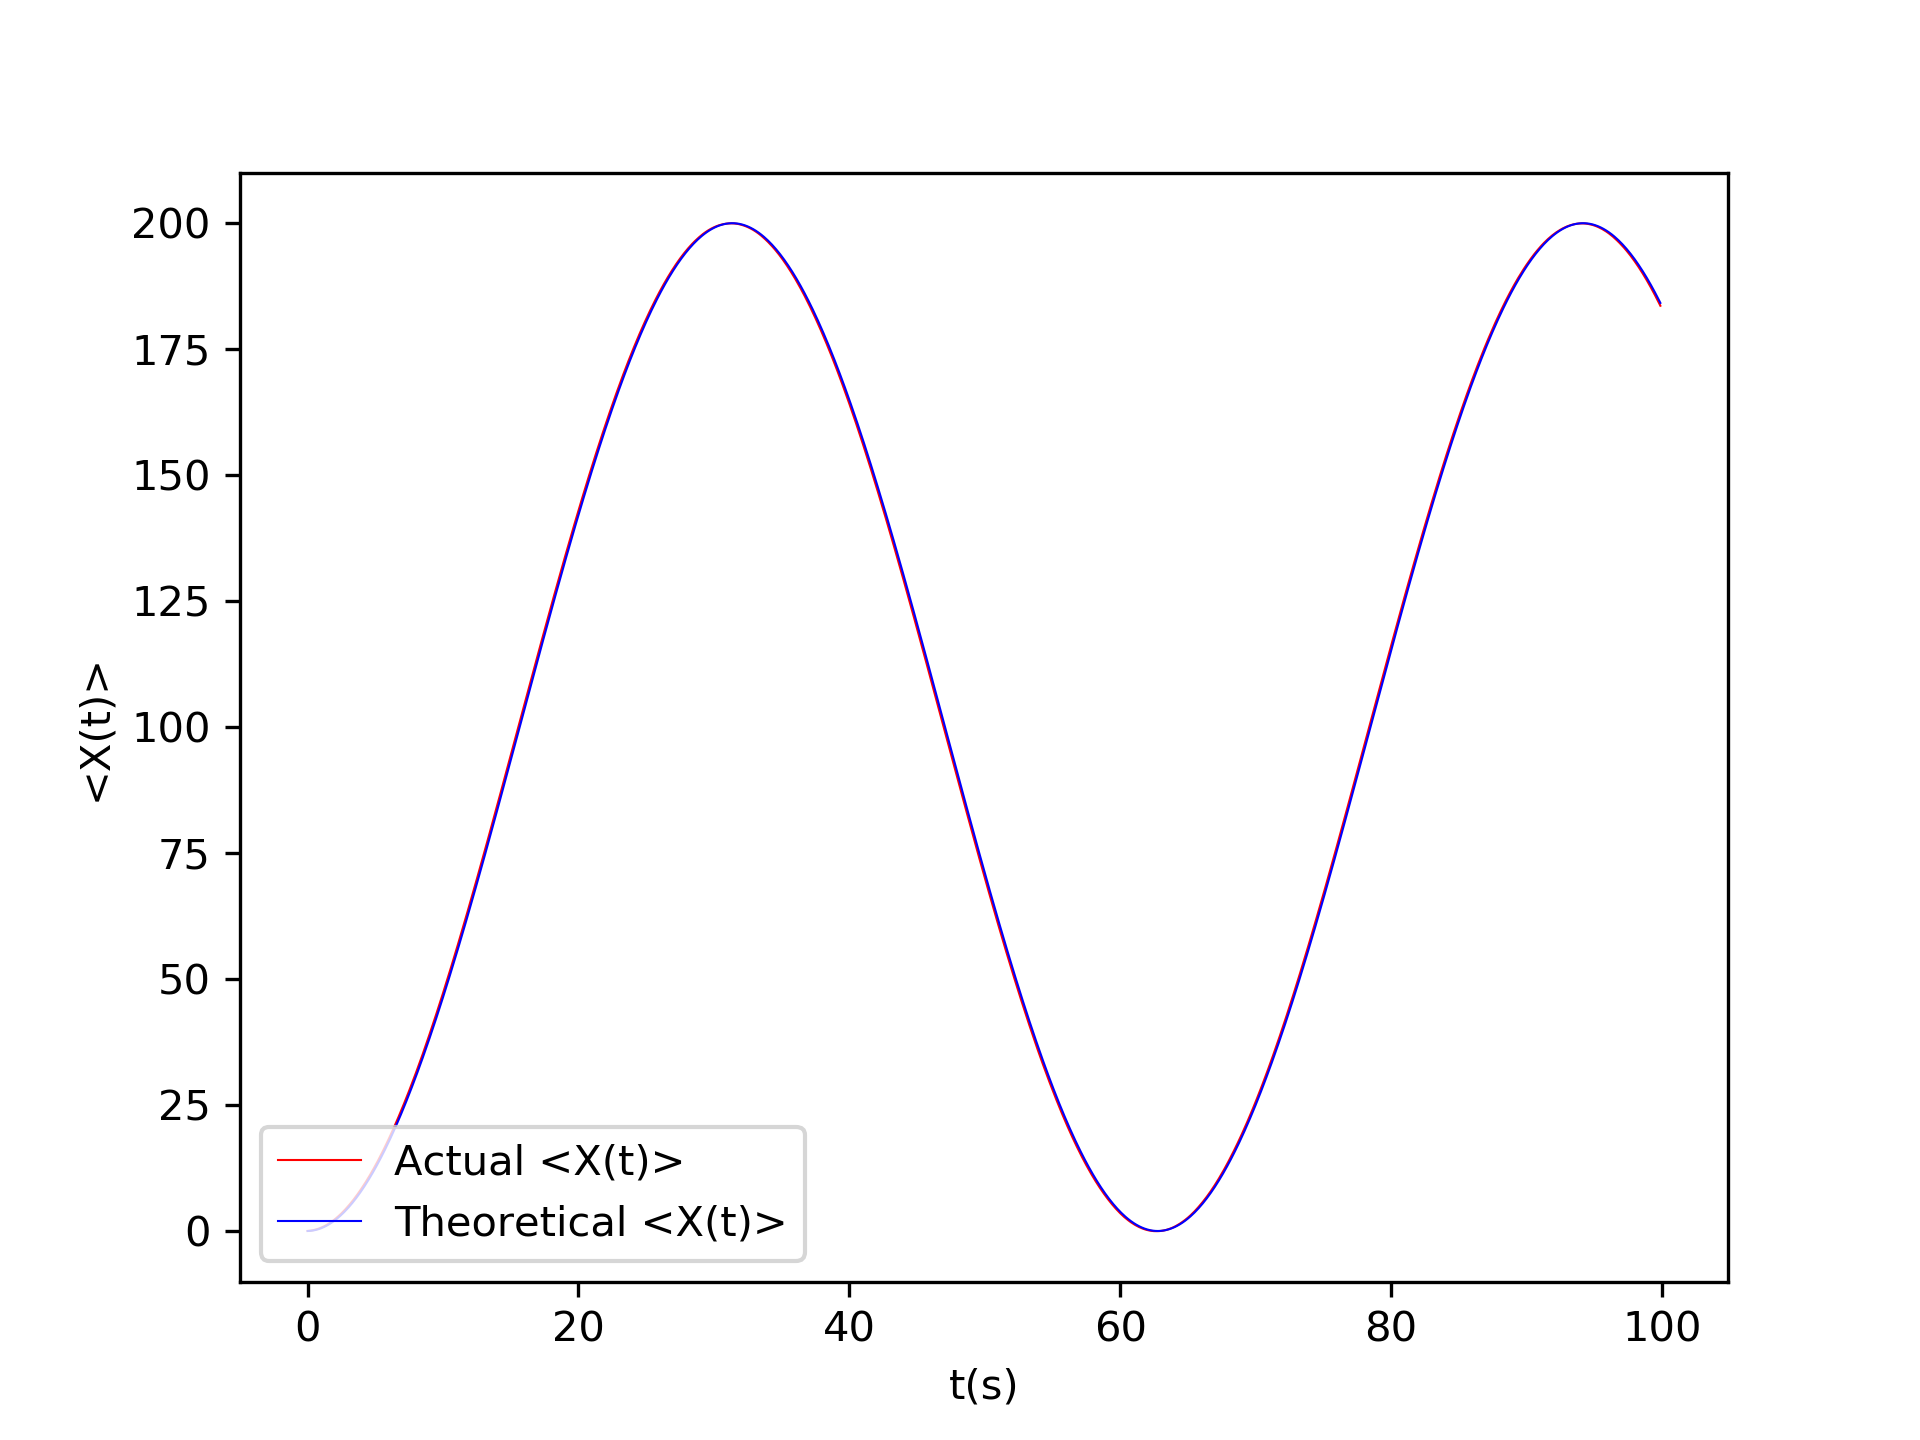
\includegraphics[bb= 0 0 450 370,width=6cm] {w=0.1/k=1-1.png}
}
\subfigure[粒子距离原点距离平方的平均]{
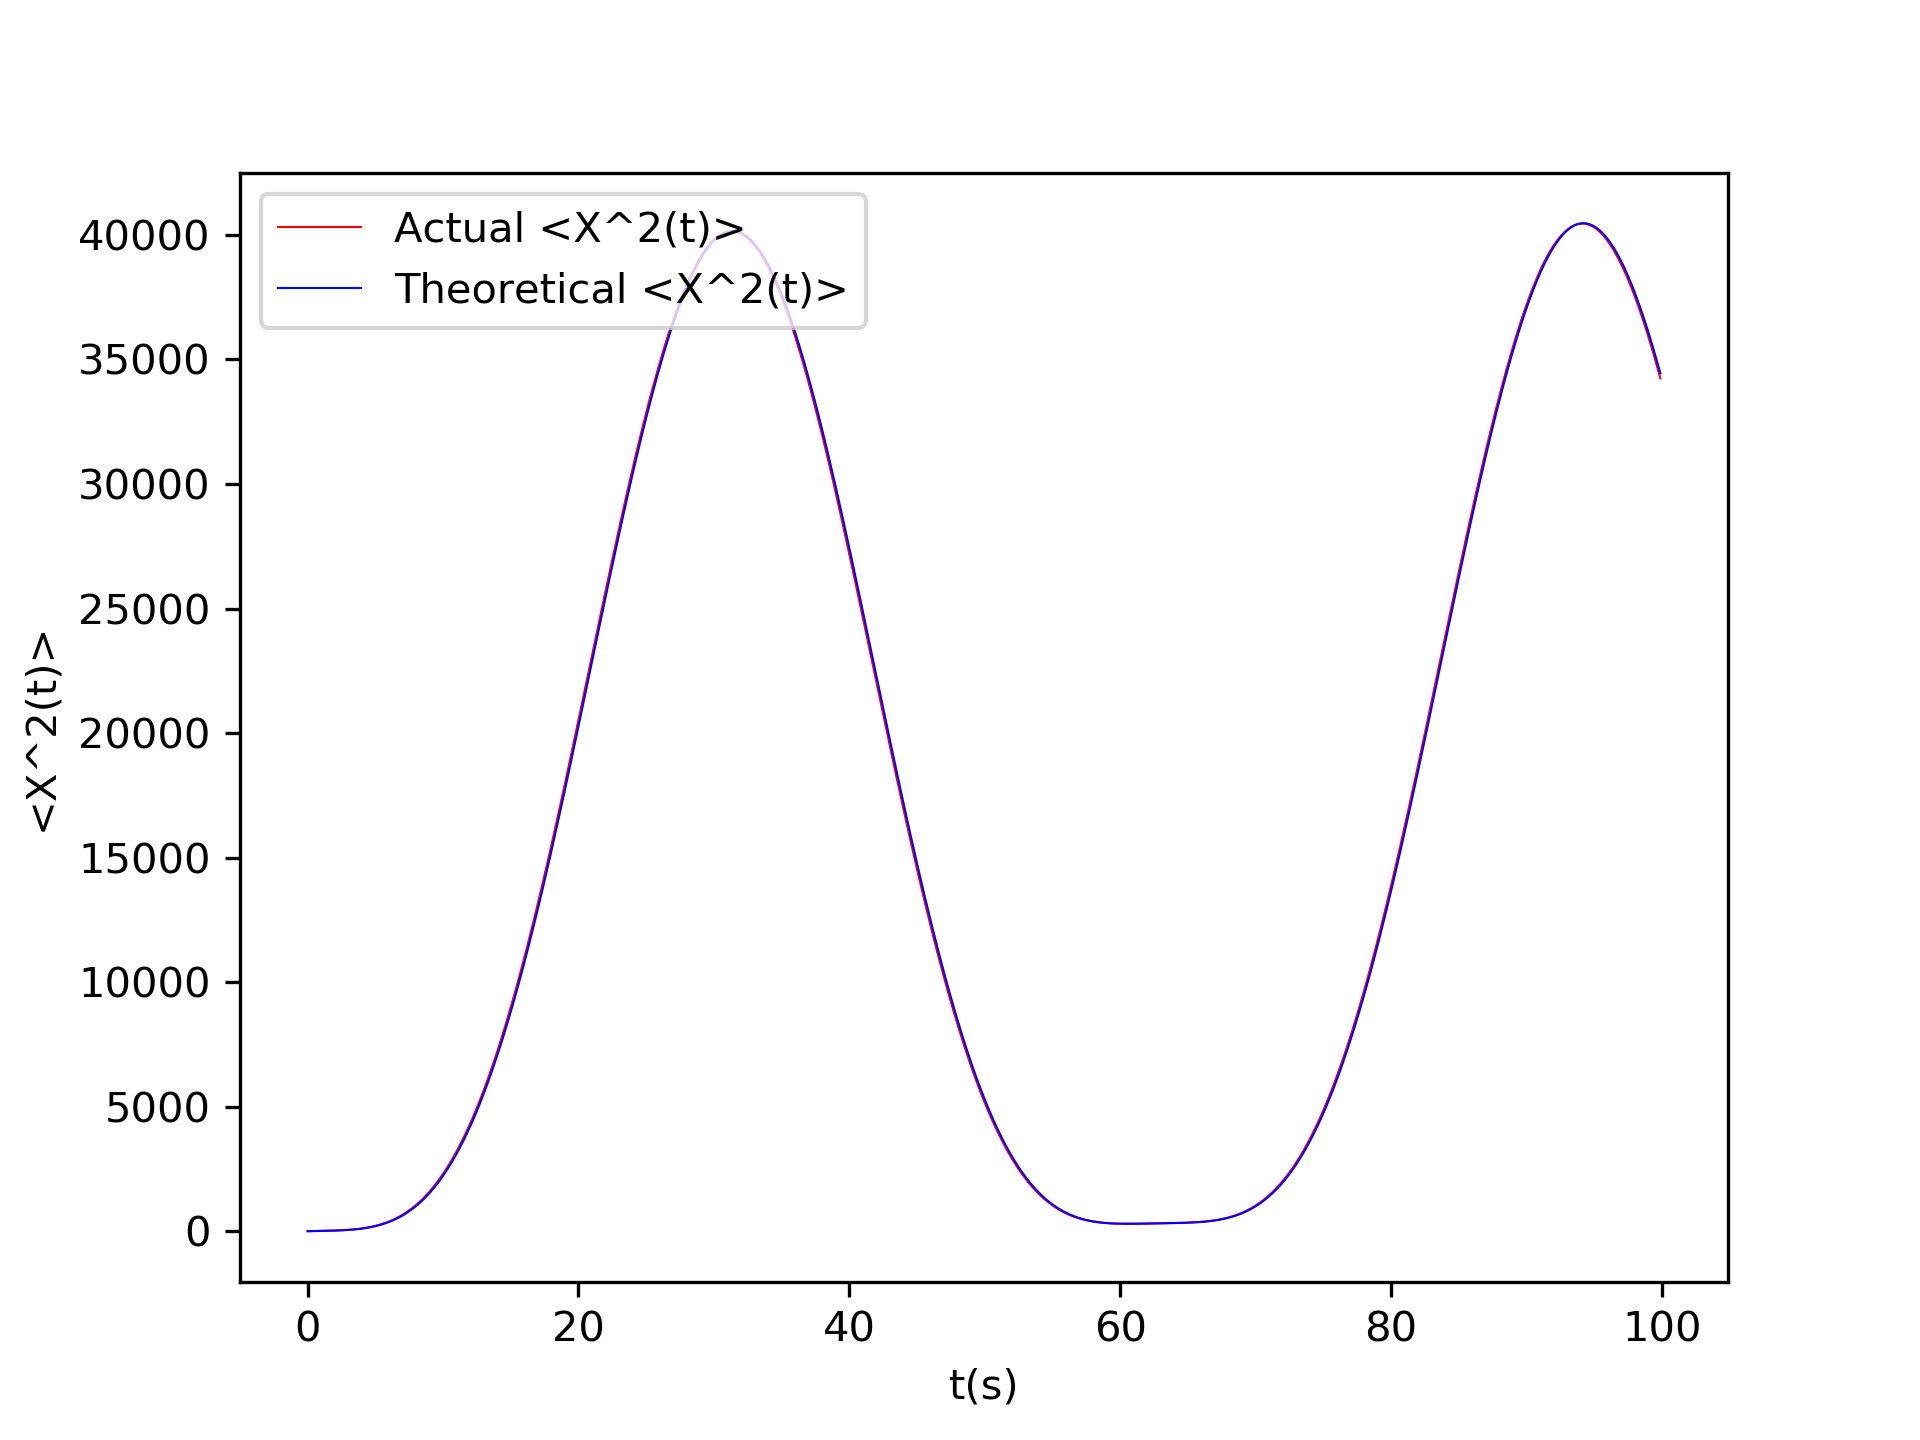
\includegraphics[bb= 0 0 450 370,width=6cm] {w=0.1/k=1-2.png}
}            
\caption{$k=1,\omega=0.1$时模拟100000个粒子行走1000步}      
\end{figure}


\begin{figure}[!htbp]   
\centering     
\subfigure[粒子的平均位置]{
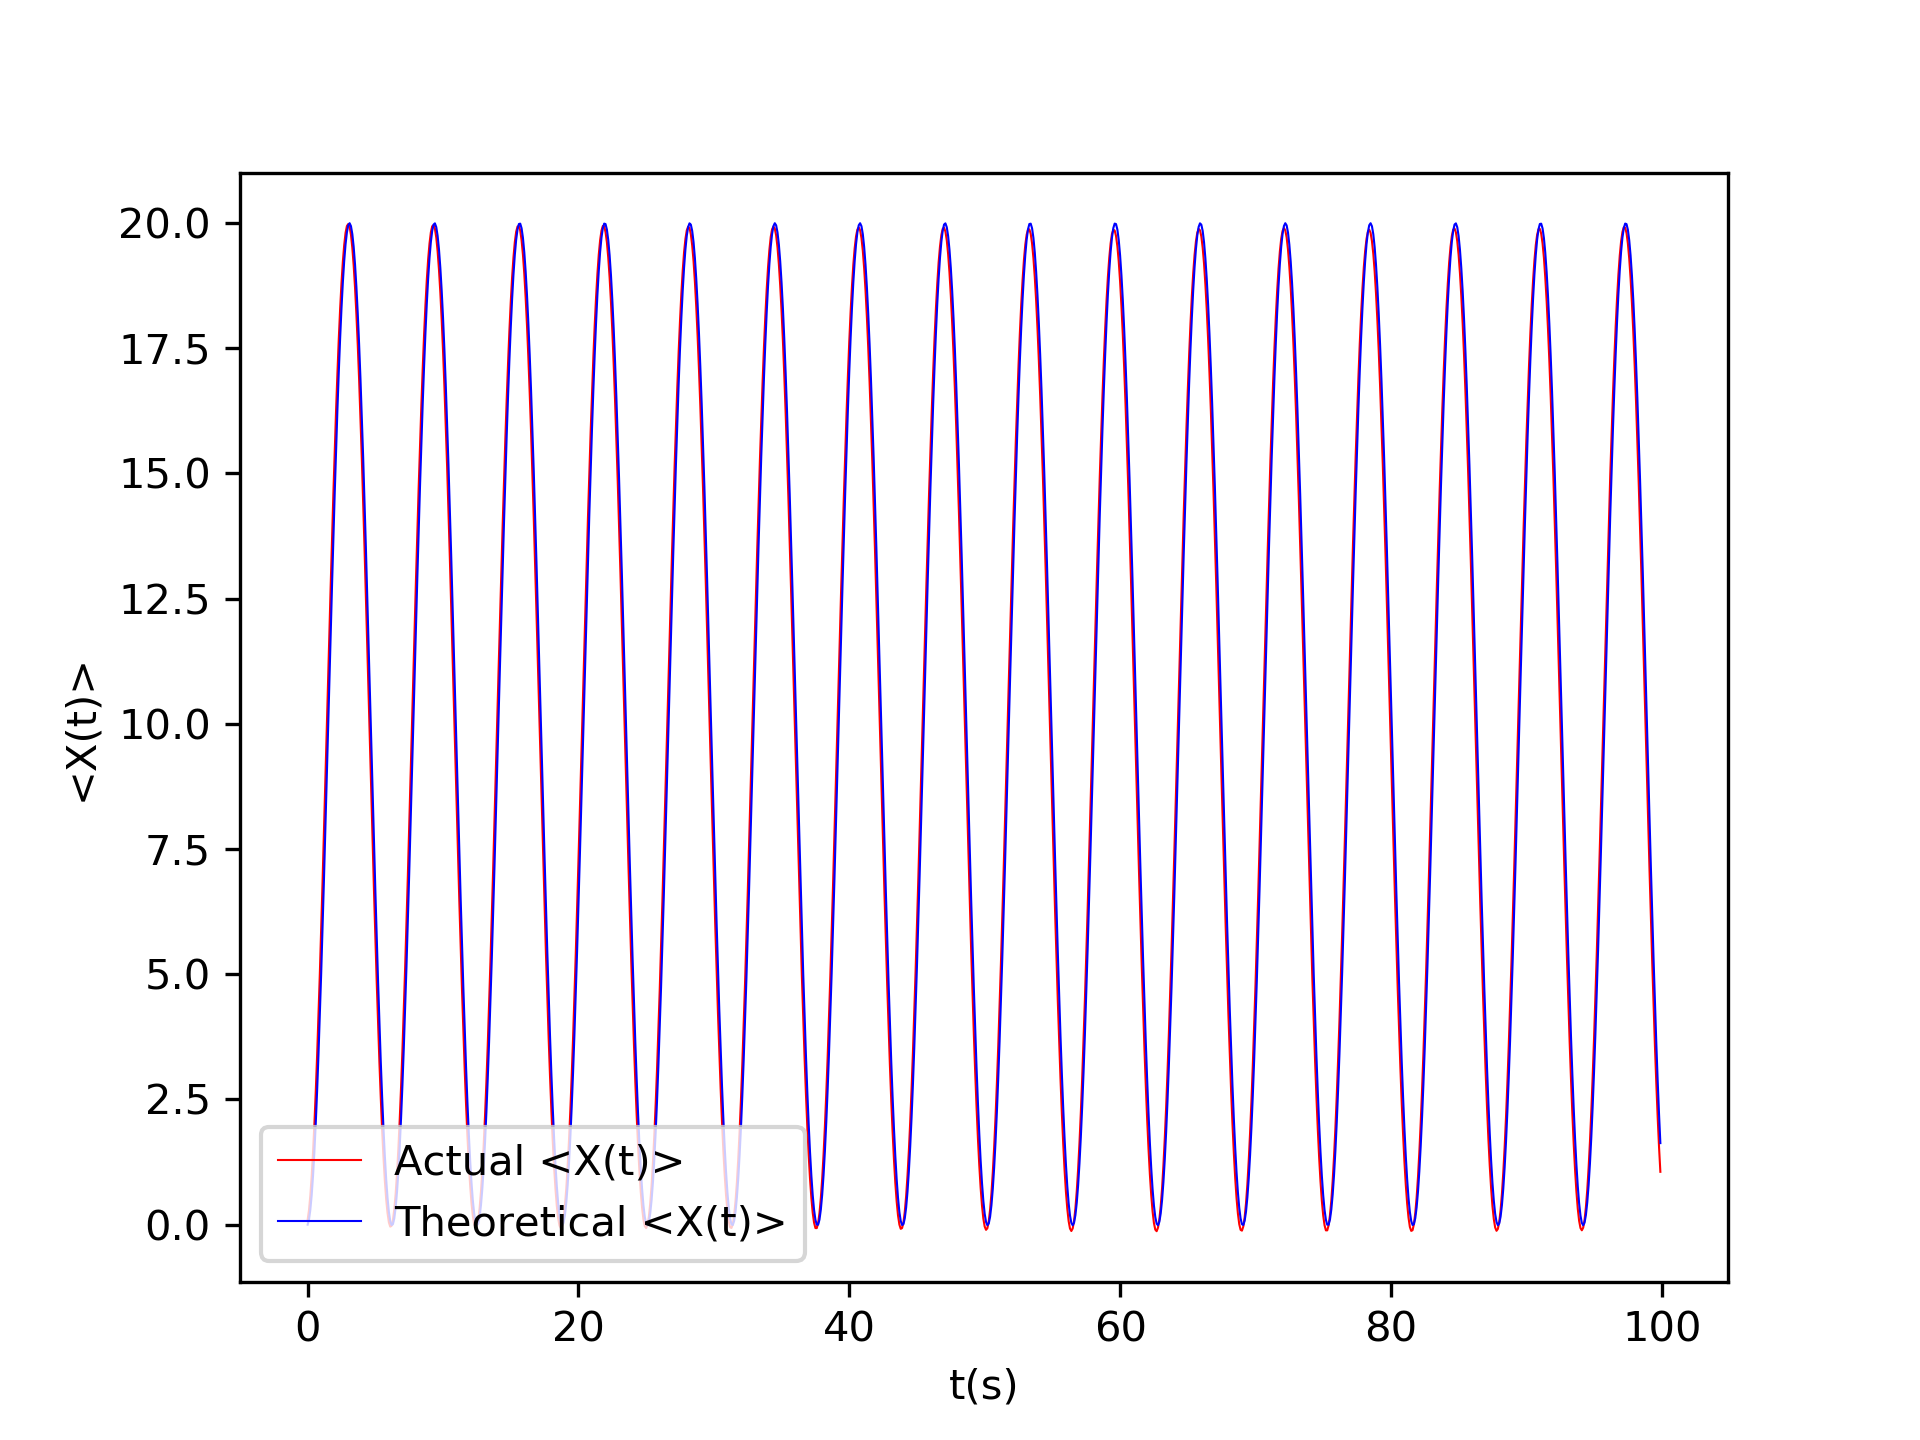
\includegraphics[bb= 0 0 450 370,width=6cm] {w=1/k=1-1.png}
}
\subfigure[粒子距离原点距离平方的平均]{
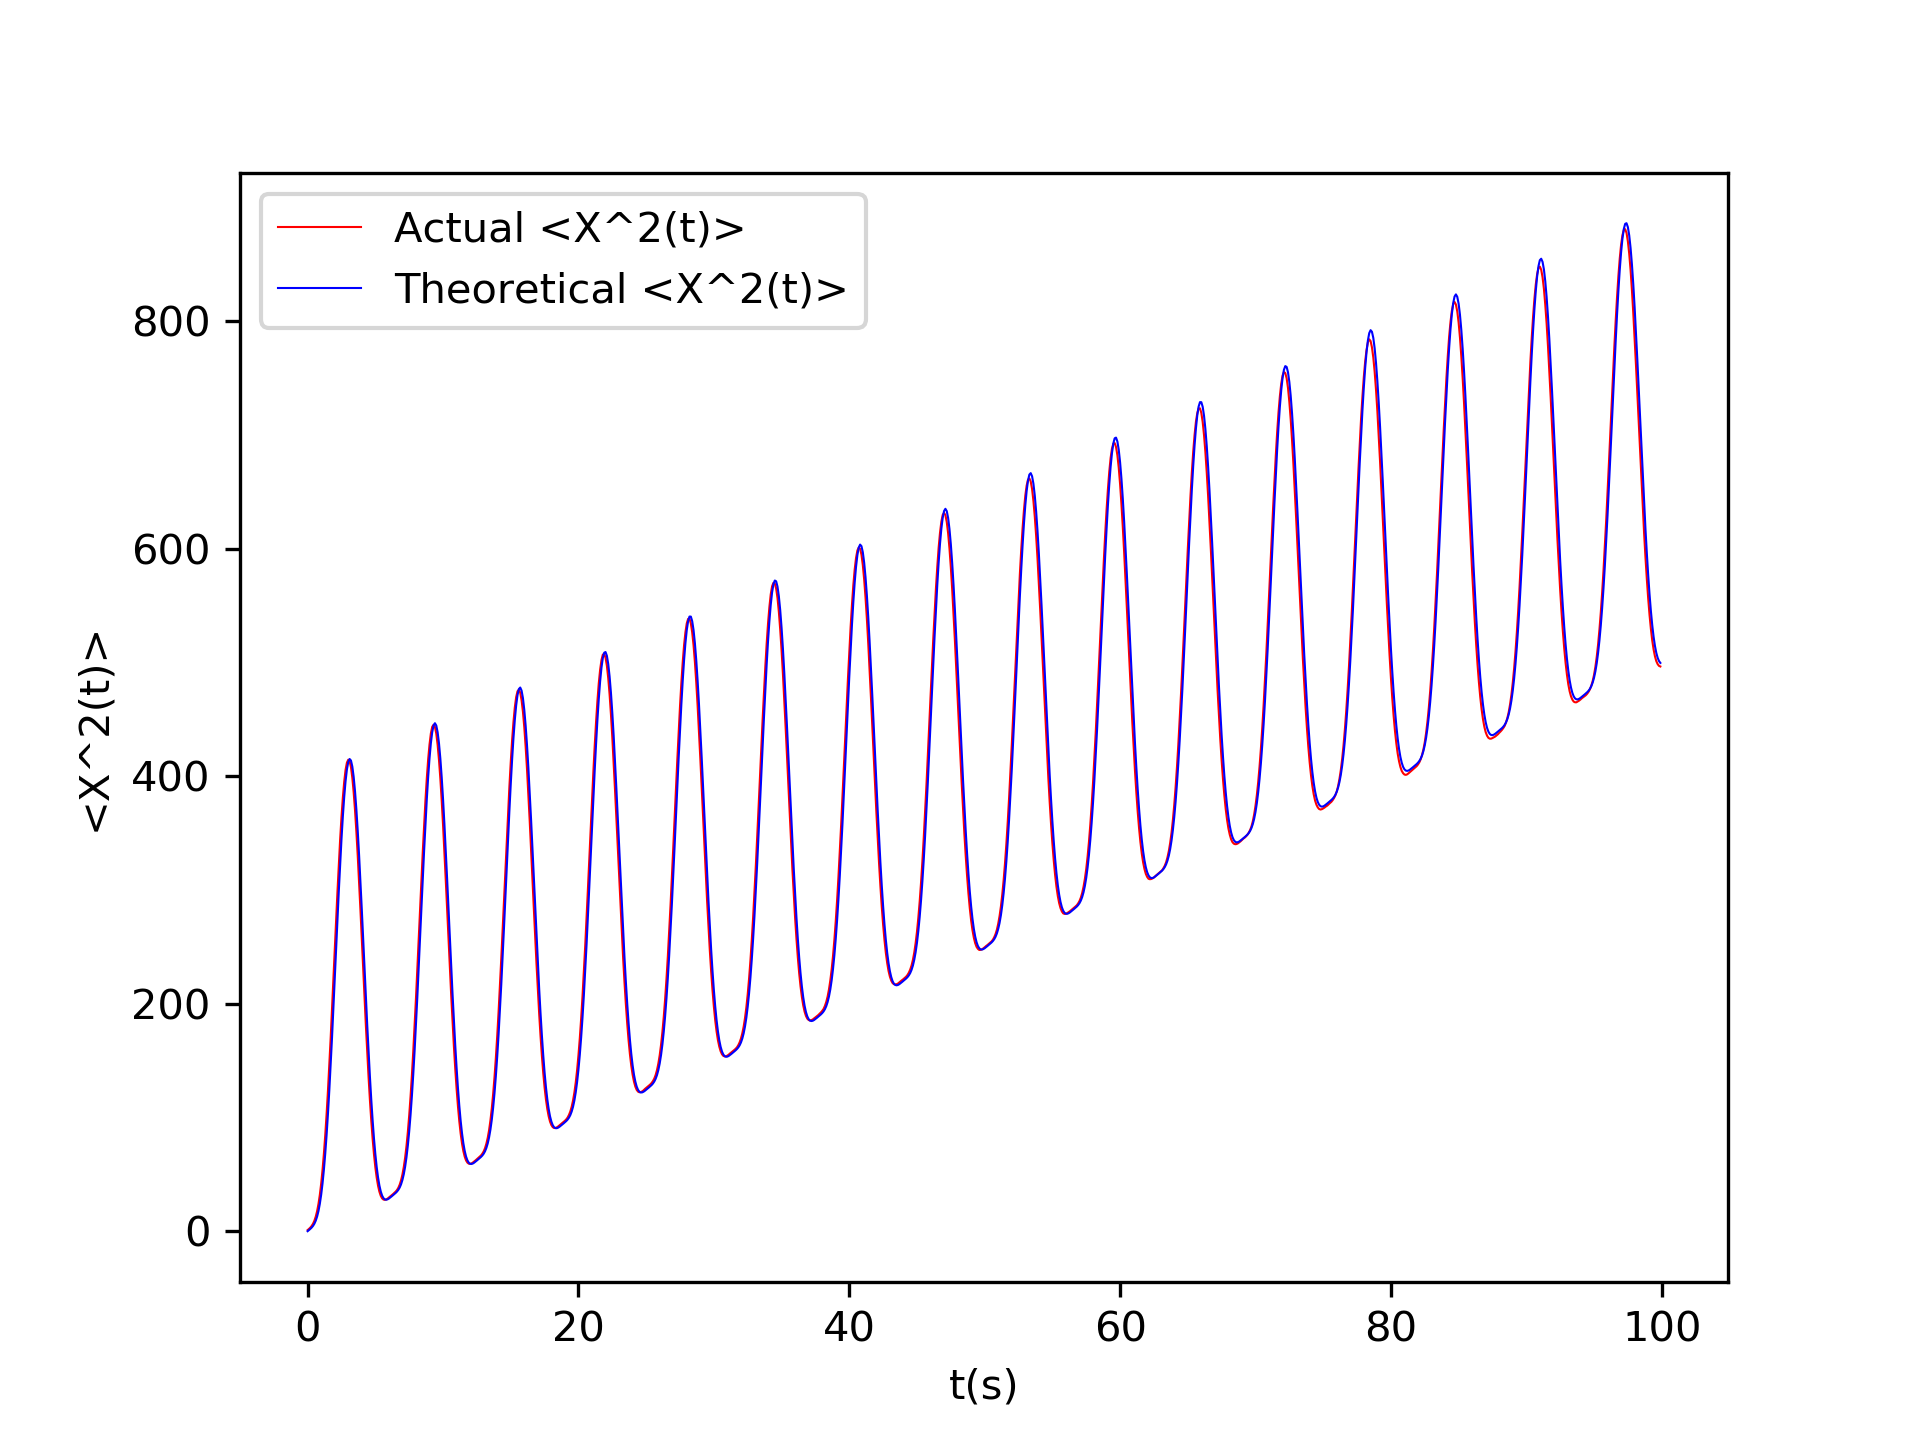
\includegraphics[bb= 0 0 450 370,width=6cm] {w=1/k=1-2.png}
}            
\caption{$k=1,\omega=1$时模拟100000个粒子行走1000步}      
\end{figure}


\begin{figure}[!htbp]   
\centering     
\subfigure[粒子的平均位置]{
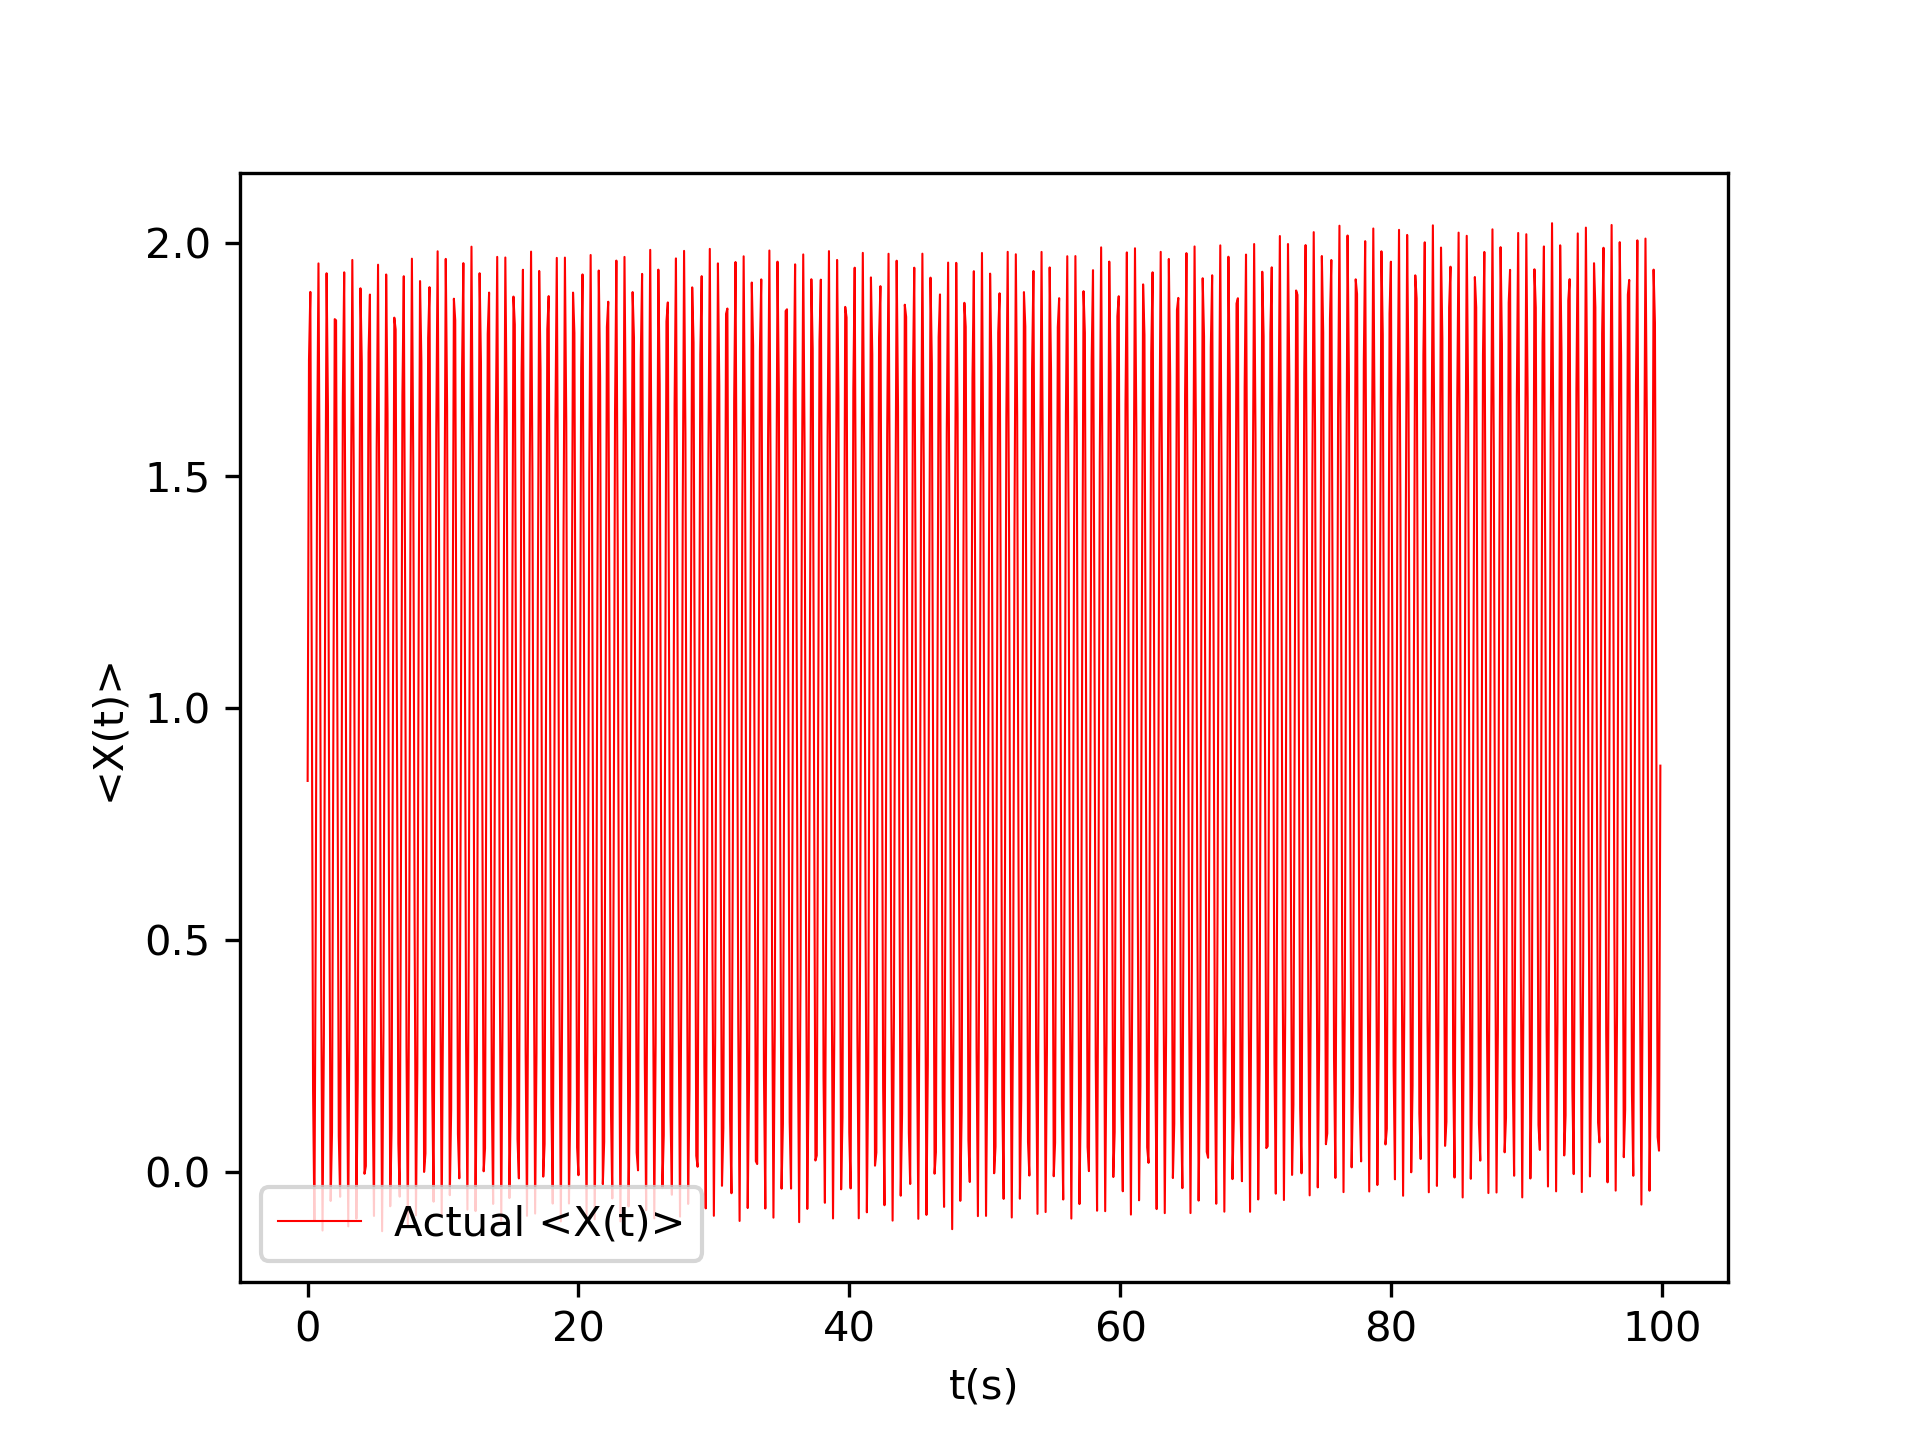
\includegraphics[bb= 0 0 450 370,width=6cm] {w=10/k=1-1.png}
}
\subfigure[粒子距离原点距离平方的平均]{
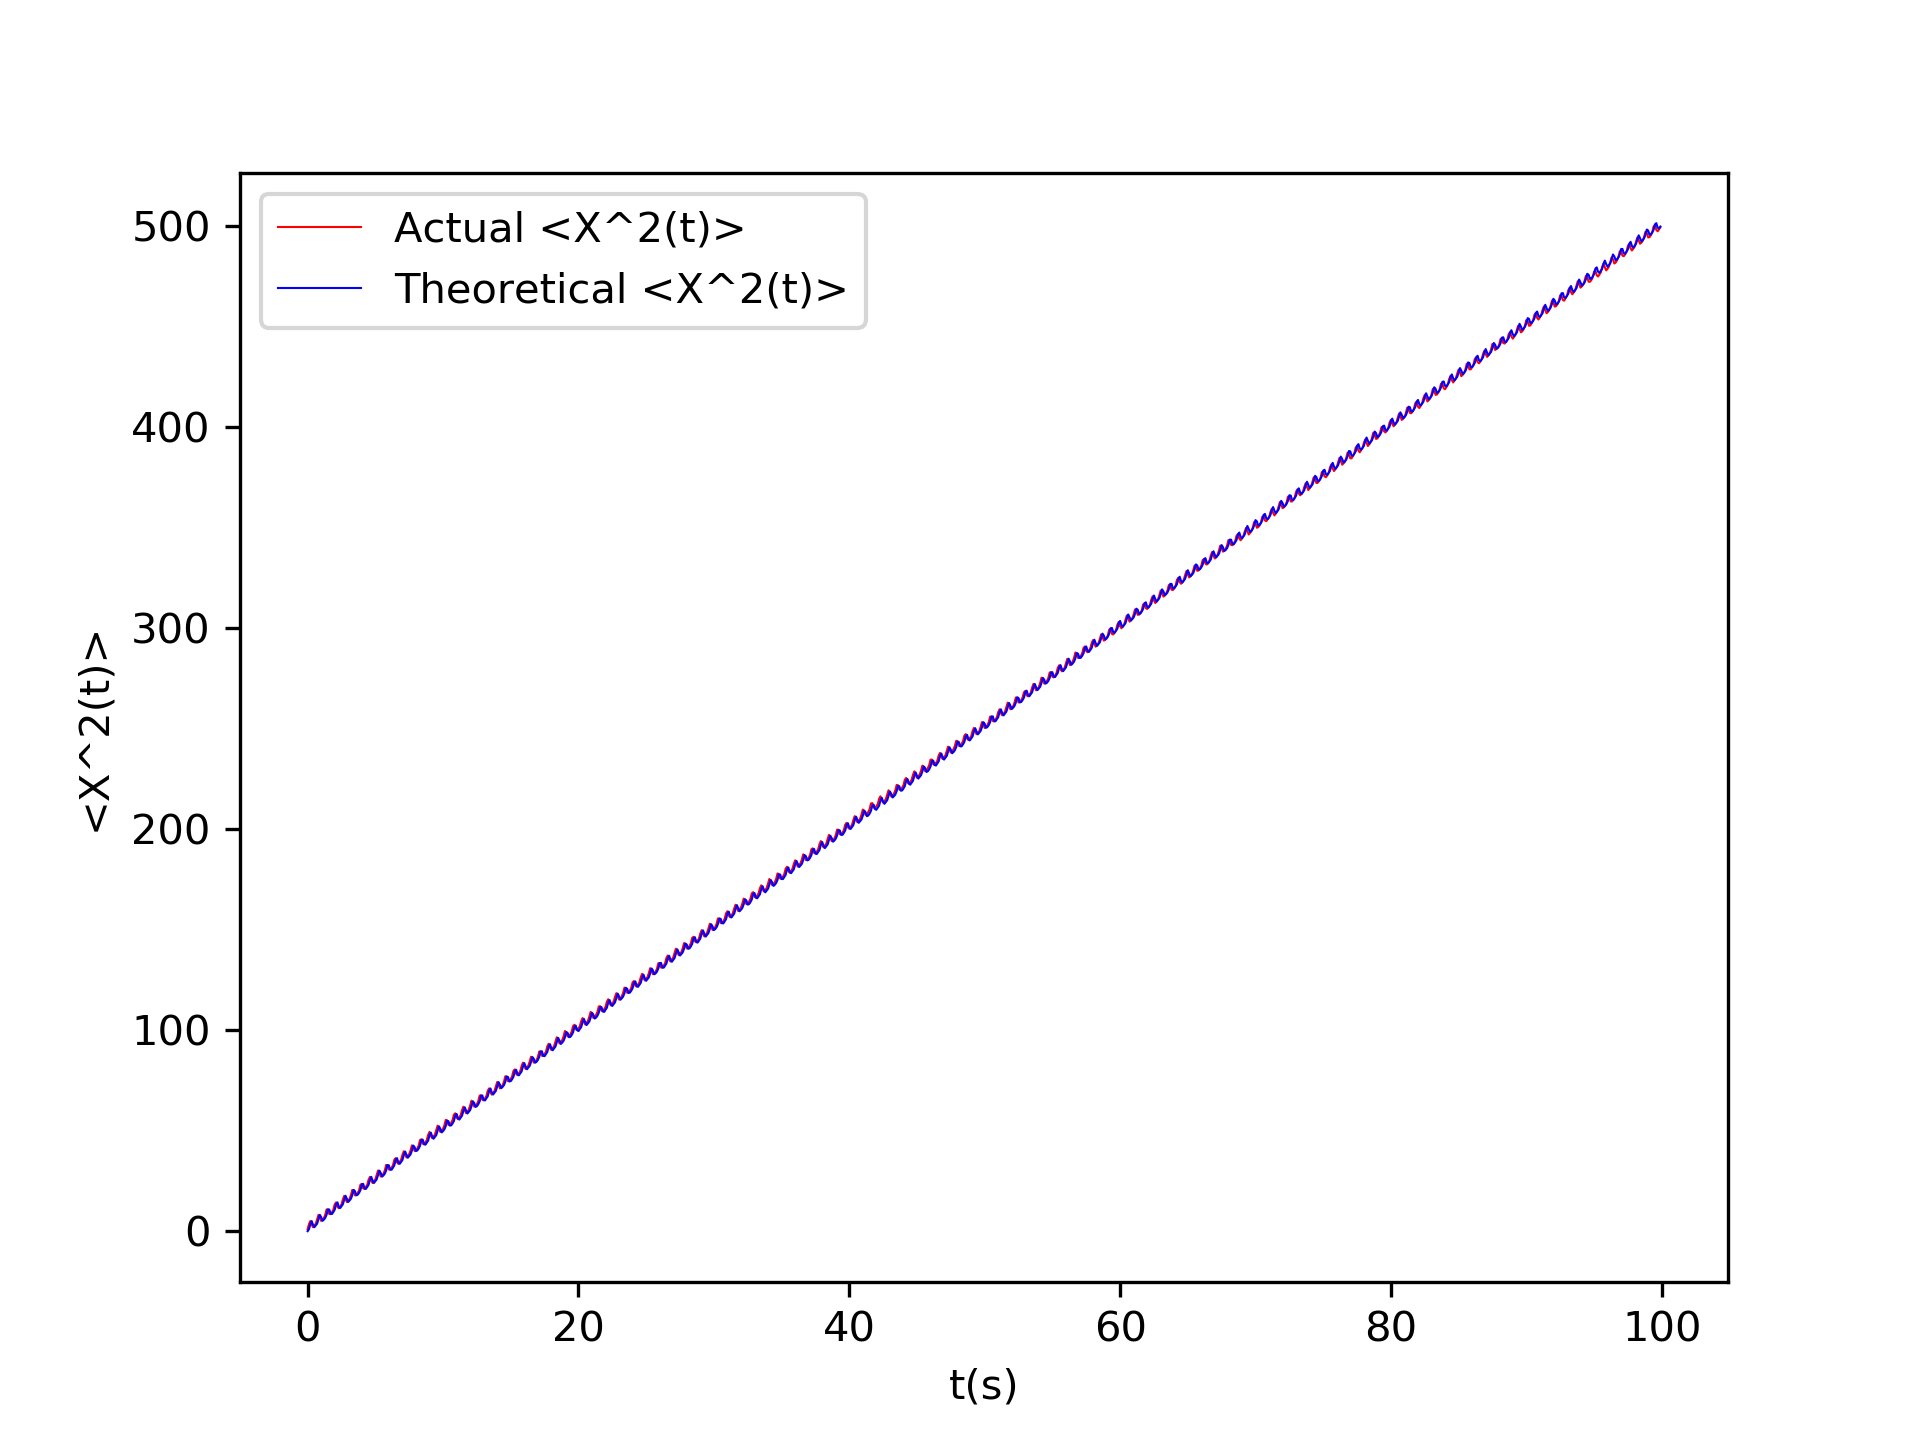
\includegraphics[bb= 0 0 450 370,width=6cm] {w=10/k=1-2.png}
}            
\caption{$k=1,\omega=10$时模拟100000个粒子行走1000步}      
\end{figure}


\begin{figure}[!htbp]   
\centering     
\subfigure[粒子的平均位置]{
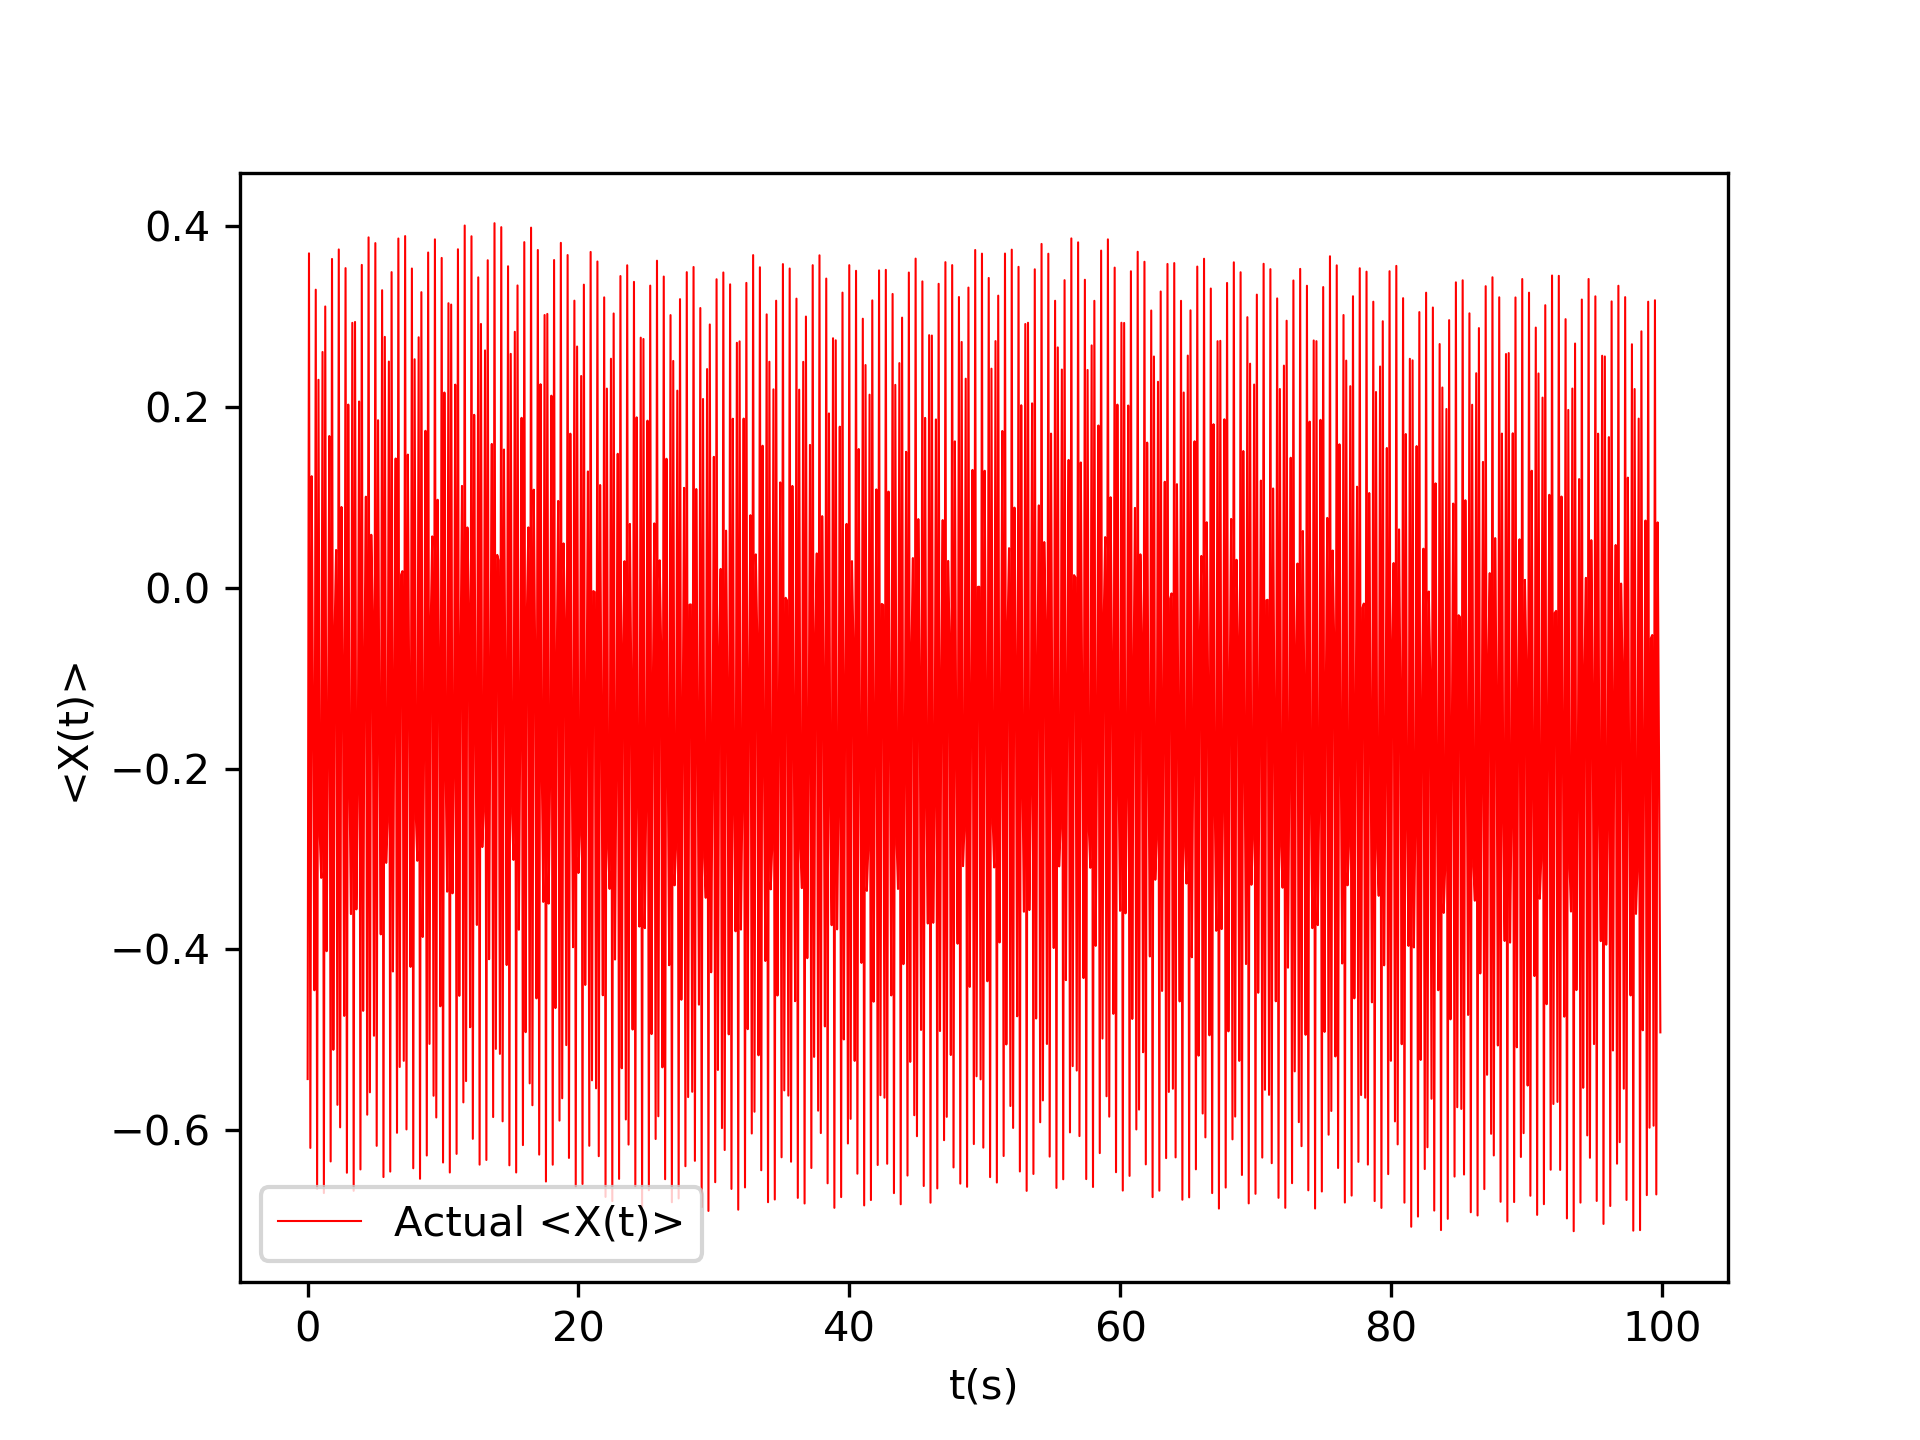
\includegraphics[bb= 0 0 450 370,width=6cm] {w=100/k=1-1.png}
}
\subfigure[粒子距离原点距离平方的平均]{
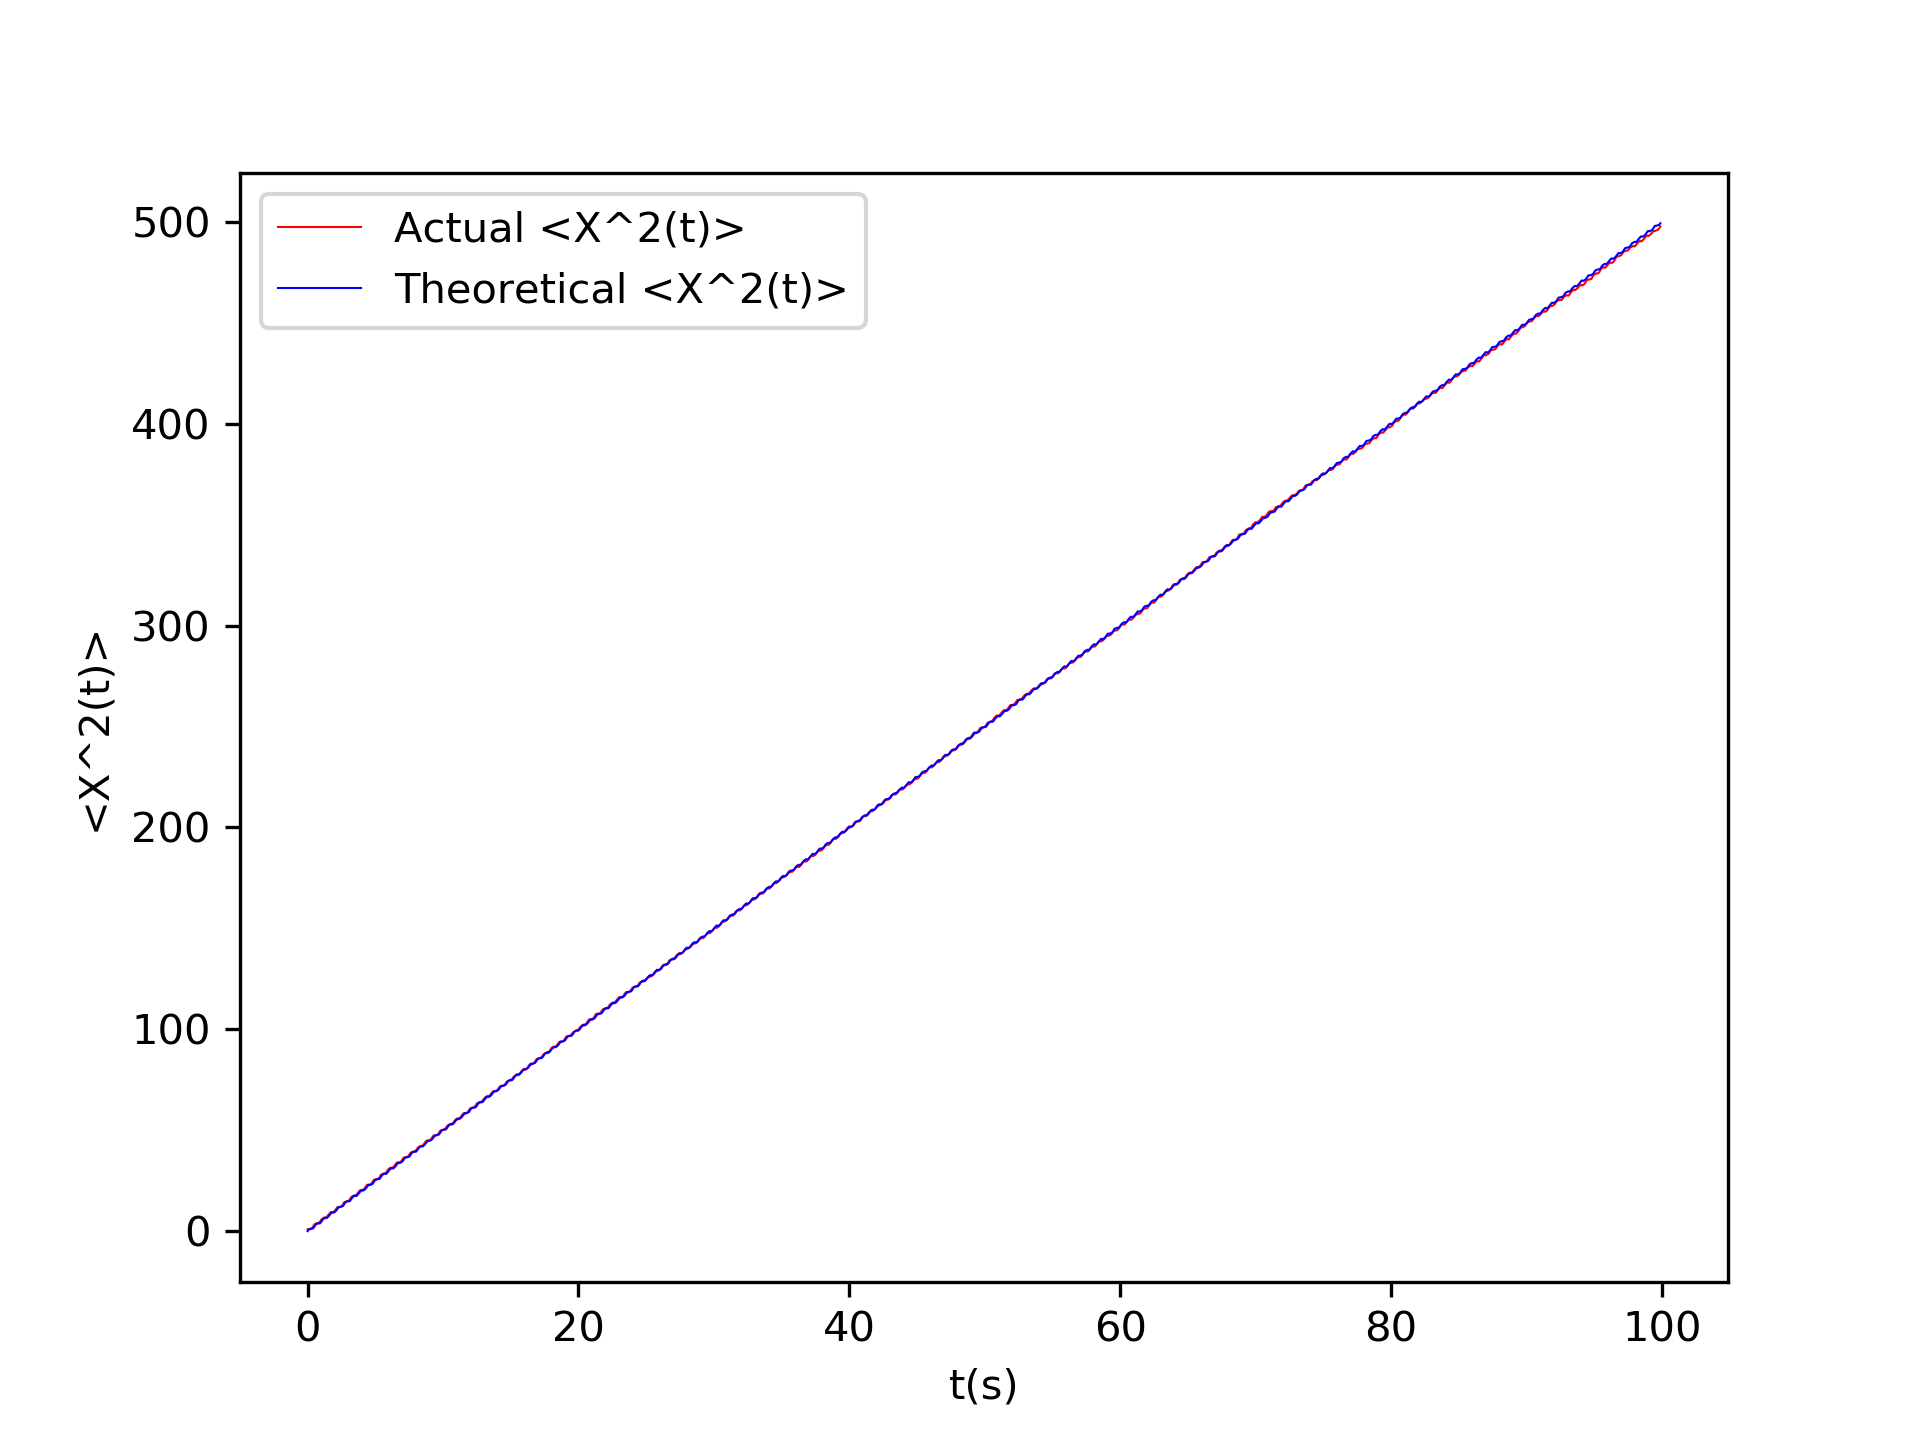
\includegraphics[bb= 0 0 450 370,width=6cm] {w=100/k=1-2.png}
}            
\caption{$k=1,\omega=100$时模拟100000个粒子行走1000步}      
\end{figure}






\newpage
 可以看出在影响因子$k=1$时粒子的平均位置已经呈现与正弦力同频率的震荡。而距离原点距离的平方的平均基本为在$k=0$时的线性关系上叠加与正弦力同频率的震荡。两者的震荡幅度均随着正弦力频率的增加而减少,与$k=0.5$时规律基本相同,但震荡幅度比同条件的$k=0.5$时的要大,这是由于此时粒子的运动受正弦力场的影响大大增强造成。
 
 
 若我们对100000个粒子行走到第1000步(取$\Delta t=0.1$,则为$t=100$时)的位置进行统计,得到:
\begin{figure}[!htbp]   
\centering
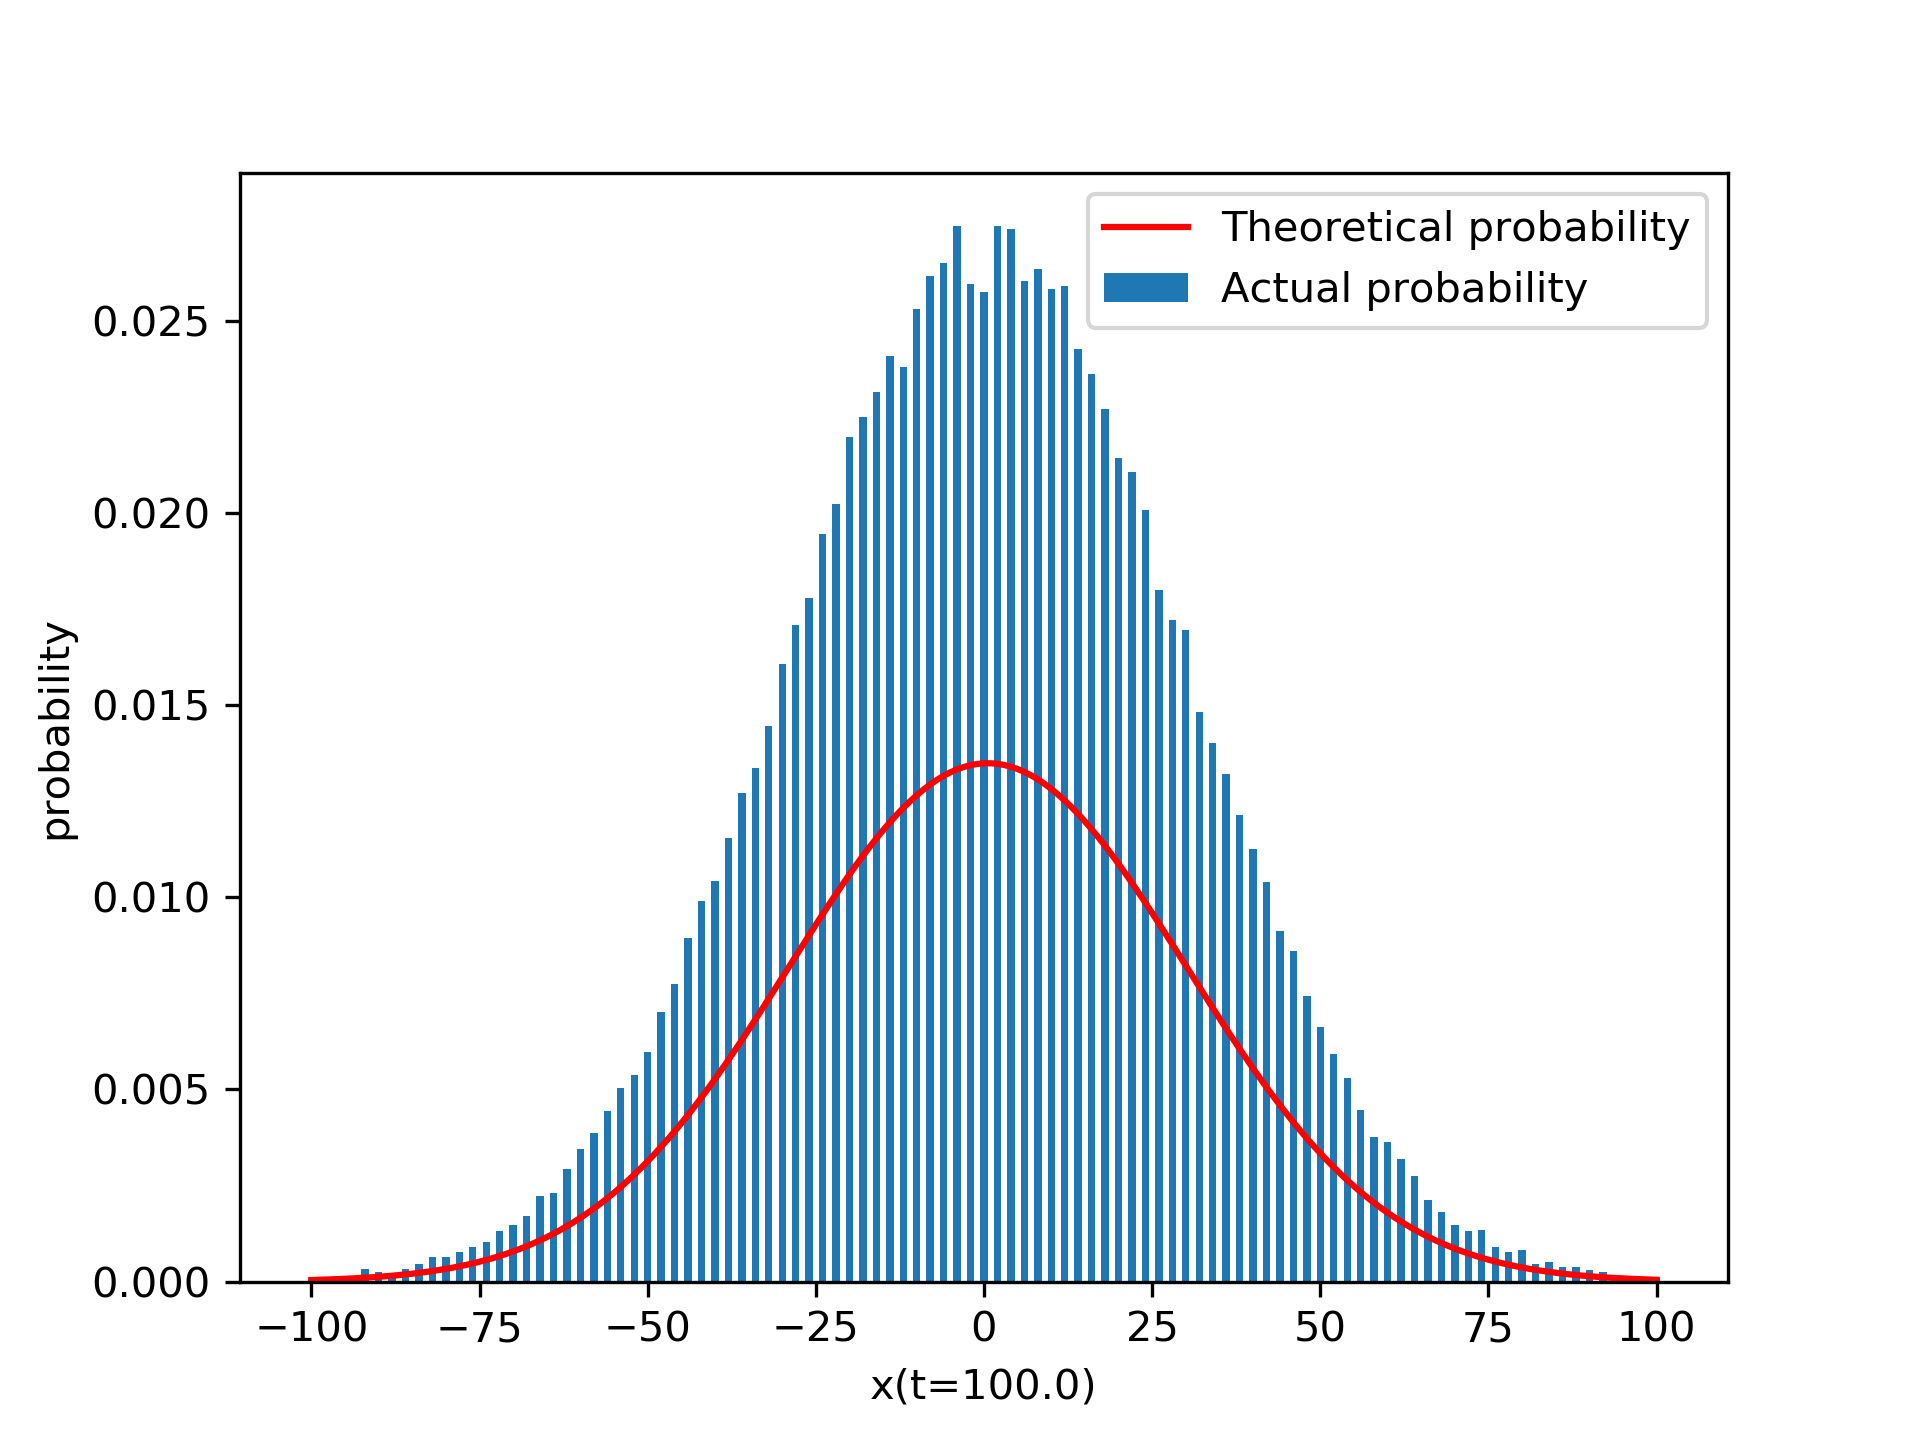
\includegraphics[bb= 0 0 450 370,width=8cm] {p-1.png}
\caption{$k=0.5,\omega=1$时模拟100000个粒子行走1000步的位置分布统计}      
\end{figure}

容易发现在奇数点的取值为0,(因为假设每一步的步长为1,故偶数步后粒子只能运动到偶数位置),故导致实际概率分布于理论概率分布差别较大。

为了修正此差别,我们将理论概率分布的值$\times 2$,与实际概率分布对比得到:
\begin{figure}[!htbp]   
\centering
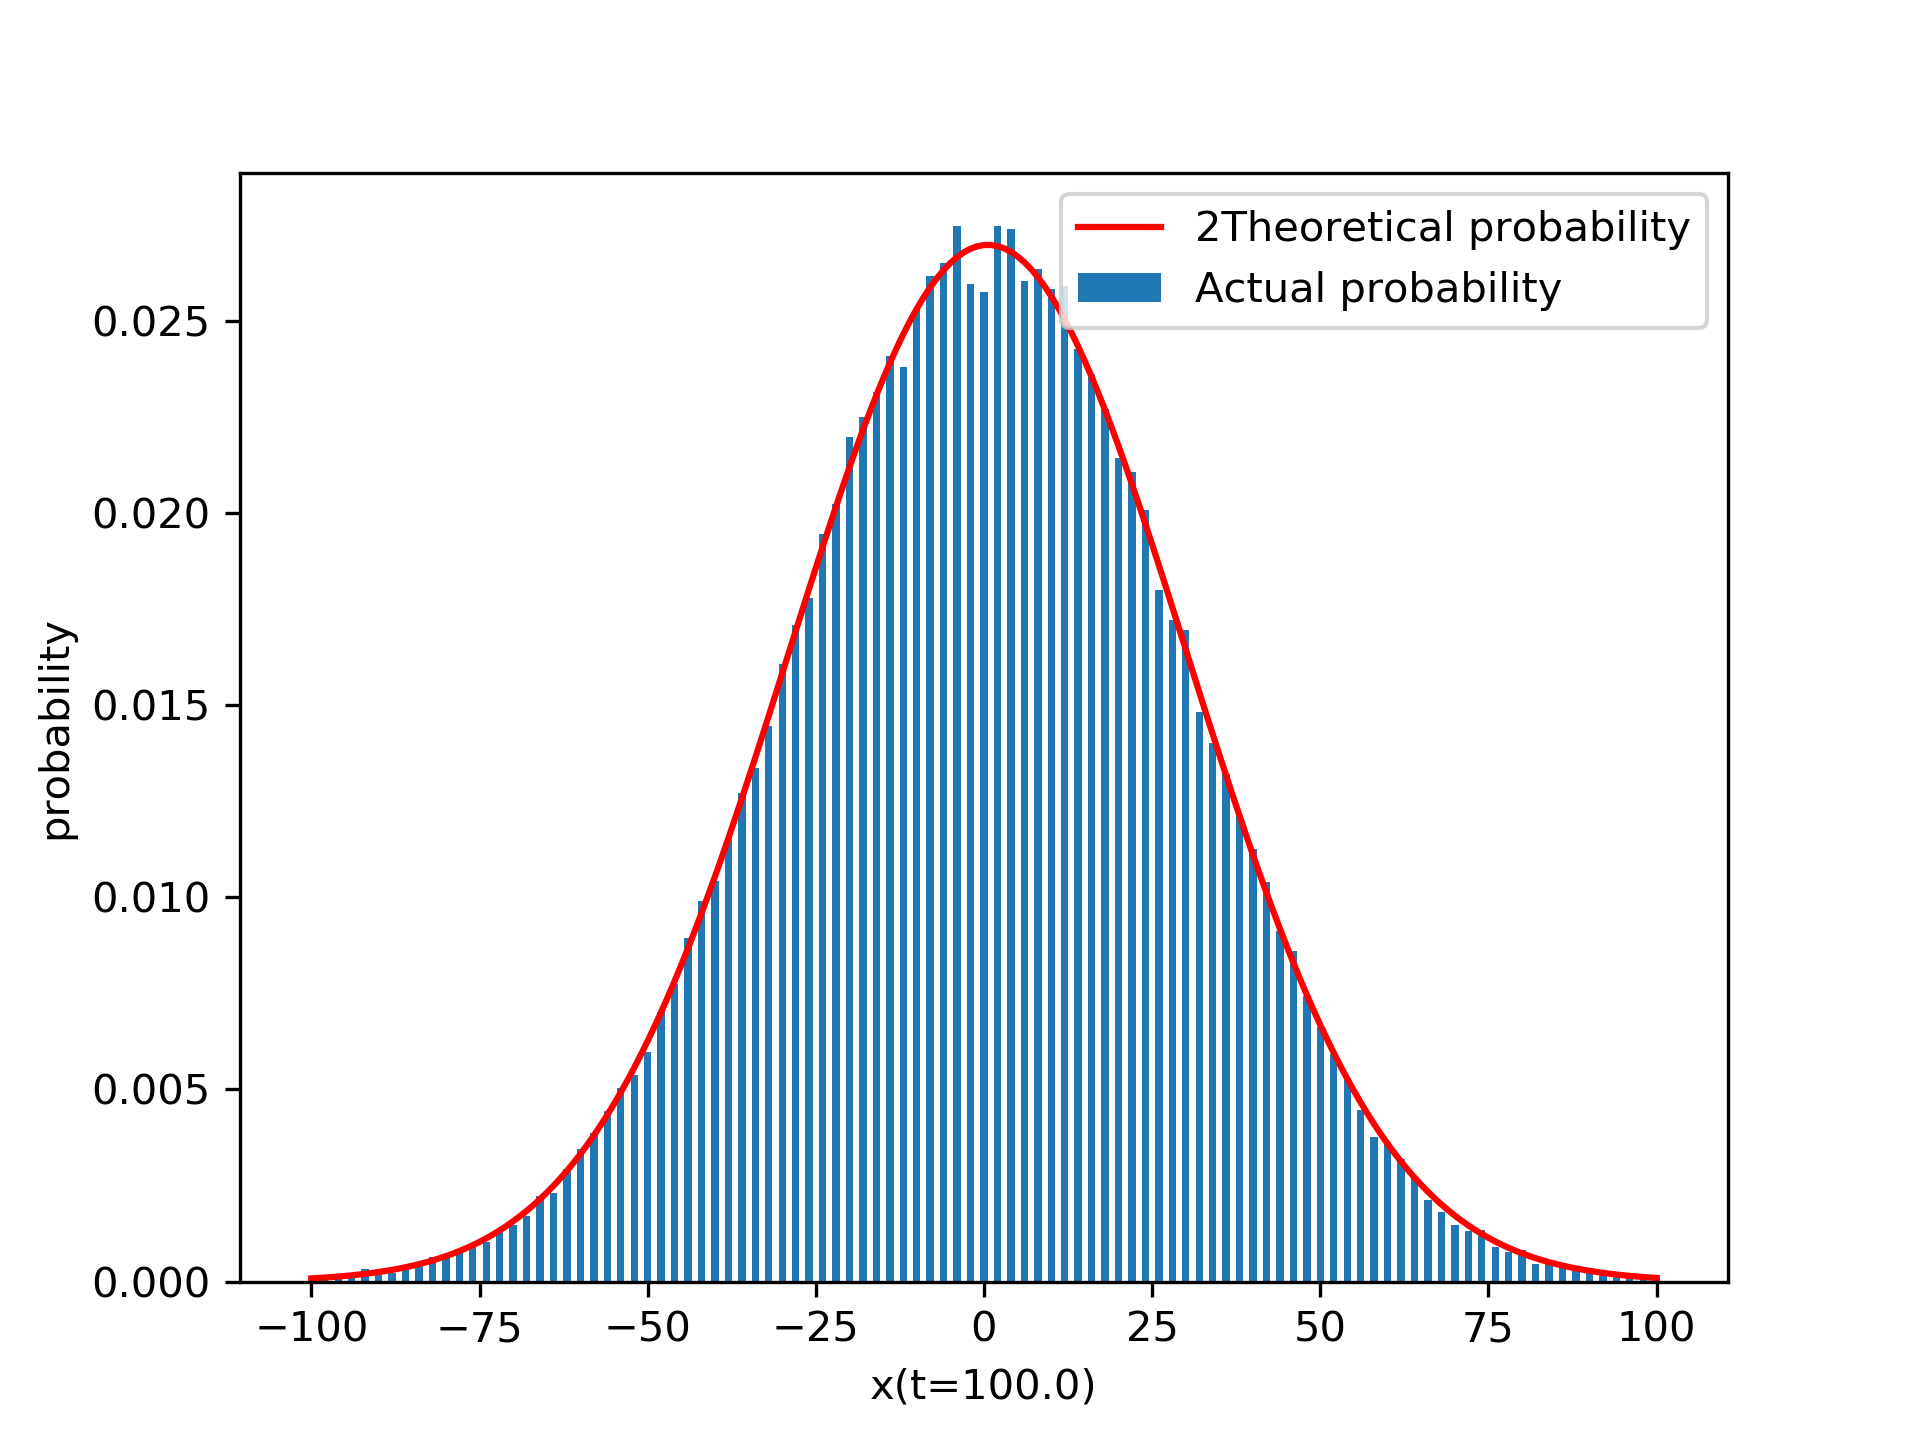
\includegraphics[bb= 0 0 450 370,width=8cm] {p-2.png}
\caption{$k=0.5,\omega=1$时模拟100000个粒子行走1000步的位置分布统计}      
\end{figure}

\newpage 可发现两者差别比较小,基本验证位置分布。
对于$t$时刻的粒子理论位置分布,有:
\begin{equation}
	p(x(t)) = \frac{1}{\sqrt{2\pi \sigma^{2}}}e^{\frac{-(x-<x(t)>)^{2}}{2\sigma^{2}}}
\end{equation}
其中$\sigma^{2}$为$x(t)$的方差。值得注意的是此理论分布是严格的二项分布的近似,不过这对于比较模拟结果足够了。严格概率分布在11题中也进行了讨论,这里不再展开叙述。
 
 
 
可以看出和计算模拟结果相差不大,差别可能是由于模拟离子不够多造成的统计涨落误差。


\section{心得与体会}
通过此次作业,对随机行走模型和布朗运动有了更深刻的认识。


\newpage
\section{附录}

\begin{appendices}


\section{C语言源程序}
\begin{lstlisting}[language = C]
#include <stdio.h>
#include <stdlib.h>
#include <math.h>
#define a 16807
#define b 0
#define m 2147483647
#define r (m%a)
#define q (m/a)
#define Pi 3.1415926
#define dt 0.1 //每步间隔时间
#define k 0.5 //影响因子的大小
#define w 1 //正弦力场的角速度大小
#define len 100  //统计概率分布时的统计范围
#define round(x) ((x)>=0?(int)((x)+0.5):(int)((x)-0.5))


//利用/dev/random 产生"真"随机数
int my_realrandom(int ran[],int n){
    FILE *fp1 = fopen("/dev/random","r");
    for(int i=0;i<n;i++){
        fread(&ran[i], 1, 4, fp1);
    }
    fclose(fp1);
    return 0;
}



int my_filewriter_double(char str1[],char str2[],double num[],int n){
    FILE * fp;
    char str[20];
    strcpy(str,str1);
    strcat(str,str2);
    fp = fopen(str,"w+");

    for(int i=0;i<(n-1);i++)
    {
        fprintf(fp,"%lf,",num[i]);

    }
    fprintf(fp,"%lf",num[n-1]);    //最后一个数据后不加 ","
    fclose(fp);
    return 0;
}



int num2str(char str[],int num){
    int  n, i = 0;
    char tmp[20];
    n = num % 10;
    while (n>0 || num > 0)
    {
        tmp[i++] = n + '0';
        num = (num - n) / 10;
        n = num % 10;
    }
    tmp[i] = '\0';
    for (i=0; i<=strlen(tmp)-1; i++)
    {
        str[i] = tmp[strlen(tmp)-i-1];
    }
    str[i] = '\0';
    return 0;
}


// Schrage 方法RW
int my_schrage_RW(double ran[],double evenx[],double evenx2[],int seed,int n,int x){
    if (seed >= 0) {
        ran[0] = seed / (double) m;
    } else {
        ran[0] = (seed + m) / (double) m;
    }
    if(seed == m-1){
        if(a >=  b){    //由于Schrage方法只对z in (0,m-1)成立,故这里要讨论z == m-1的情况
            seed = m + (b-a) % m;
        }
        else   seed =  (b-a) % m;

    }
    
    else seed = ((a * (seed % q) - r * (seed /  q)) + b % m ) % m;  //递推式
    if (ran[0] < 0.5*( 1 - k*sin(w*dt)) )
        ran[0] = -1;
    else ran[0] = 1;
    evenx[0] += ran[0]/x;
    evenx2[0] += pow(ran[0],2)/x;
   
    for (int i = 1; i < n-1; i++) {
        if (seed >= 0) {
            ran[i] = seed / (double) m;
        } else {
            ran[i] = (seed + m) / (double) m;
        }
        if(seed == m-1){
            if(a >=  b){    //由于Schrage方法只对z in (0,m-1)成立,故这里要讨论z == m-1的情况
                seed = m + (b-a) % m;
            }
            else   seed =  (b-a) % m;

        }
        else seed = ((a * (seed % q) - r * (seed /  q)) + b % m ) % m;  //递推式
        if (ran[i] < 0.5*( 1 - k*sin(w*(i+1)*dt)) )
            ran[i] = ran[i-1]- 1;
        else ran[i] = ran[i-1] + 1;
        evenx[i] += ran[i]/x;
        evenx2[i] += pow(ran[i],2)/x;
    }
    
    
    if (seed >= 0) {
        ran[n-1] = seed / (double) m;
    } else {
        ran[n-1] = (seed + m) / (double) m;
    }
    if (ran[n-1] < 0.5*( 1 - k*sin(w*n*dt)) )
        ran[n-1] = ran[n-2]- 1;
    else ran[n-1] = ran[n-2] + 1;
    evenx[n-1] += ran[n-1]/x;
    evenx2[n-1] += pow(ran[n-1],2)/x;
    
    return 0;
}






int main(int argc, const char * argv[]) {
    int N;    //总随机数个数(总步长k个数)
    int n;    //总粒子个数
    int flag = 0; //是否输出每个模拟粒子每步的位置数据文件
    char str[50];
    printf("请输入您所需要的总步数:");
    while (!scanf("%d",&N)){   //简单的输入检查
        gets(str);
        printf("\nInput error,please try again\n");
        printf("请输入您所需要的总步数:");
    }
    
    printf("请输入您所需总粒子个数:");
    while (!scanf("%d",&n)){   //简单的输入检查
        gets(str);
        printf("\nInput error,please try again\n");
        printf("请输入您所需要的总粒子个数:");
    }
    
    printf("是否输出每个模拟粒子的位置数据至文件?是输1,不是输0:");
    while (!scanf("%d",&flag)){   //简单的输入检查
        gets(str);
        printf("\nInput error,please try again\n");
        printf("是否输出每个模拟粒子的位置数据至文件?是输1,不是输0:");
    }

    if(N*n >1000000) printf("您输入的参数已接受,正在计算请稍等片刻~\n");

    double *ran = malloc(sizeof(double) * N);  //用来存放每个粒子每一步的位置
    double *evenx = malloc(sizeof(double) * N);  //用来存放所有粒子每一步位置的平均值
    double *evenx2 = malloc(sizeof(double) * N);  //用来存放所有粒子每一步位置平方的平均值
    double *p = malloc(sizeof(double)*(2*len+1));
    double *var = malloc(sizeof(double)*N);
    int *seed = malloc(sizeof(int) * n);  //用来存放随机种子值
    
    my_realrandom(seed, n);
    

    for(int i=0;i<N;i++){  //对evenx进行初始化
        evenx[i] = 0;
        evenx2[i] = 0;
        var[i] = 0;
    }
    
    for(int i=0;i <= 2*len;i++){  //对evenx进行初始化
        p[i] = 0;
    }
    
    
    char str1[10];
    for(int i = 0;i<n;i++){
        num2str(str1,i+1);
        my_schrage_RW(ran,evenx,evenx2,seed[i],N,n);
        p[round(ran[N-1]) + len]  += (double)1/n;
        if(flag == 1 && n < 20 ) my_filewriter_double(str1, "RW.dat", ran, N);
    }
    num2str(str1, n);
    for(int i=0;i<N;i++){
        var[i] = (evenx2[i]-pow(evenx[i],2))/n;
    }
    my_filewriter_double(str1, "evenx.dat", evenx, N);
    my_filewriter_double(str1, "evenx2.dat", evenx2, N);
    my_filewriter_double(str1, "p.txt", p, (2*len+1));
    my_filewriter_double(str1, "var.txt", var, N);
    return 0;
}

\end{lstlisting}

\newpage

\section{可视化绘图python程序源码}

\begin{lstlisting}[language = python]

import matplotlib.pyplot as plt
from mpl_toolkits.mplot3d import Axes3D
import numpy as np
#from IPython.core.pylabtools import figsize # import figsize
#figsize(12.5, 4) # 设置 figsize
plt.rcParams['savefig.dpi'] = 300 #图片像素
plt.rcParams['figure.dpi'] = 300 #分辨率
# 默认的像素:[6.0,4.0],分辨率为100,图片尺寸为 600&400
fig1 = plt.figure()
fig2 = plt.figure()
fig = plt.figure()
pfig = plt.figure()
figvar = plt.figure()
ax1 = fig1.add_subplot(111)
ax2 = fig2.add_subplot(111)
ax = fig.add_subplot(111)
pax = pfig.add_subplot(111)
axvar = figvar.add_subplot(111)

n = 5
N = 1000
dt = 0.1
w = 1
k = 0

X = []
Y1 = []
Y2 = []
p = []
var = []

with open('problem 10/w='+str(w)+'/'+str(N)+'evenx_'+str(k)+'.dat', 'r') as f:
    while True:
        lines = f.readline() # 整行读取数据
        if not lines:
            break
        Y1 = [float(i) for i in lines.split(',')]  # 将整行数据分割处理
    Y1 = np.array(Y1) # 将数据从list类型转换为array类型。

with open('problem 10/w='+str(w)+'/'+str(N)+'evenx2_'+str(k)+'.dat', 'r') as f:
    while True:
        lines = f.readline() # 整行读取数据
        if not lines:
            break
        Y2 = [float(i) for i in lines.split(',')]  # 将整行数据分割处理
    Y2 = np.array(Y2) # 将数据从list类型转换为array类型。


with open('problem 10/'+str(100000)+'p.txt', 'r') as f:
    while True:
        lines = f.readline() # 整行读取数据
        if not lines:
            break
        p = [float(i) for i in lines.split(',')]  # 将整行数据分割处理
    p = np.array(p) # 将数据从list类型转换为array类型。


with open('problem 10/'+str(10000)+'var.txt', 'r') as f:
    while True:
        lines = f.readline() # 整行读取数据
        if not lines:
            break
        var = [float(i) for i in lines.split(',')]  # 将整行数据分割处理
    var = np.array(var) # 将数据从list类型转换为array类型。


Y2 = np.sqrt(Y2*Y2)
X = np.arange(0, N * dt, dt)
px = np.arange(-100, 101, 1)
varx = np.arange(0, 10000, 1)
print(np.shape(px))
py = 1/np.sqrt(2*np.pi*875.265)*np.exp(-np.power(px-0.56124, 2)/(2*875.265))


ax1.plot(X, Y1, 'b', label='<X(t)>', lw=0.3)
ax1.set_xlabel('t(s)')
ax1.set_ylabel('<X(t)>')
fig1.savefig("1.png")

axvar.plot(varx, var, 'b', label='<X(t)>', lw=0.3)
axvar.set_xlabel('t(s)')
axvar.set_ylabel('var(t)')
figvar.savefig("var.png")


ax2.plot(X, Y2, 'b', label='<X^2(t)>', lw=0.3)
ax2.set_xlabel('t(s)')
ax2.set_ylabel('<X^2(t)>')
fig2.savefig("2.png")

pax.bar(px, p, width=1.1, label='Actual probability')
pax.plot(px, py, 'r', label='Theoretical probability')
pax.set_xlabel('x(t='+str(N*dt)+')')
pax.set_ylabel('probability')
pax.legend(loc=1)
pfig.savefig("p.png")

Y = [[]]
Y = np.array(Y)

for i in range(n):
    with open('problem 10/'+str(i+1)+'RW.dat', 'r') as f:
        while True:
            lines = f.readline()  # 整行读取数据
            if not lines:
                break
            Y = np.append(Y, [[float(i) for i in lines.split(',')]])  # 将整行数据分割处理

Y = Y.reshape(n, N)

plt_label = 0
for link in range(n):
    ax.plot(X, Y[link], label='particle'+str(plt_label), lw=0.3)
    plt_label += 1

ax.set_xlabel('t(s)')
ax.set_ylabel('X(t)')
fig.savefig("3.png")


\end{lstlisting}


\end{appendices}




\end{document}
